% ------------------------------------------------------------------------
% ------------------------------------------------------------------------
% abnTeXf2: Modelo de Trabalho Academico (tese de doutorado, dissertacao de
% mestrado e trabalhos monograficos em geral) em conformidade com 
% ABNT NBR 14724:2011: Informacao e documentacao - Trabalhos academicos -
% Apresentacao
% ------------------------------------------------------------------------
% ------------------------------------------------------------------------

\documentclass[
	% -- opções da classe memoir --
	12pt,				% tamanho da fonte
	openright,			% capítulos começam em pág ímpar (insere página vazia caso preciso)
	oneside,			% para impressão em verso e anverso. Oposto a oneside
	a4paper,			% tamanho do papel. 
	% -- opções da classe abntex2 --
	%chapter=TITLE,		% títulos de capítulos convertidos em letras maiúsculas
	%section=TITLE,		% títulos de seções convertidos em letras maiúsculas
	%subsection=TITLE,	% títulos de subseções convertidos em letras maiúsculas
	%subsubsection=TITLE,% títulos de subsubseções convertidos em letras maiúsculas
	% -- opções do pacote babel --
	english,			% idioma adicional para hifenização
	french,				% idioma adicional para hifenização
	spanish,			% idioma adicional para hifenização
	brazil,				% o último idioma é o principal do documento
	oldfontcommands
	]{abntex2}

% ---
% Pacotes básicos 
% ---
\usepackage{lmodern}			% Usa a fonte Latin Modern			
\usepackage[T1]{fontenc}		% Selecao de codigos de fonte.
\usepackage[utf8]{inputenc}		% Codificacao do documento (conversão automática dos acentos)
\usepackage{lastpage}			% Usado pela Ficha catalográfica
\usepackage{indentfirst}		% Indenta o primeiro parágrafo de cada seção.
\usepackage{color}				% Controle das cores
\usepackage{graphicx}			% Inclusão de gráficos
\usepackage{microtype} 			% para melhorias de justificação
\usepackage{eurosym}			% habilita símbolo do Euro
\usepackage{amsmath}
% ---
		
% ---
% Pacotes adicionais, usados apenas no âmbito do Modelo Canônico do abnteX2
% ---
%\usepackage{lipsum}				% para geração de dummy text
% ---

% ---
% Pacotes de citações
% ---
\usepackage[brazilian,hyperpageref]{backref}	 % Paginas com as citações na bibl
\usepackage[num]{abntex2cite}	% Citações padrão ABNT


% --- 
% CONFIGURAÇÕES DE PACOTES
% --- 

% ---
% Configurações do pacote backref
% Usado sem a opção hyperpageref de backref
\renewcommand{\backrefpagesname}{Citado na(s) página(s):~}
% Texto padrão antes do número das páginas
\renewcommand{\backref}{}
% Define os textos da citação
\renewcommand*{\backrefalt}[4]{
	\ifcase #1 %
		Nenhuma citação no texto.%
	\or
		Citado na página #2.%
	\else
		Citado #1 vezes nas páginas #2.%
	\fi}%
% ---

% ---
% Informações de dados para CAPA e FOLHA DE ROSTO
% ---
\titulo{SISTEMA DE GERENCIAMENTO DE ENERGIA PARA CUBESATS}
\autor{ARNALDO ALVES VIANA JÚNIOR\\
OTÁVIO MOREIRA PETITO\\
TIAGO AUGUSTO ORCAJO DEMAY CORDEIRO}
\local{São Caetano do Sul}
\data{2015}
\orientador{Prof. Me. Alessandro de Oliveira Santos}
%\coorientador{Professor}
\instituicao{Escola de Engenharia Mauá}
%tipotrabalho{Tese (Trabalho de Conclusão de Curso)}
% O preambulo deve conter o tipo do trabalho, o objetivo, 
% o nome da instituição e a área de concentração 
\preambulo{Trabalho de Conclusão de Curso apresentado à Escola de Engenharia Mauá do Centro Universitário do Instituto Mauá de Tecnologia, como parte dos requisitos necessários à obtenção do grau de bacharel em Engenharia na habilitação Engenharia Eletrônica. Área de concentração: Engenharia Elétrica}
% ---


% ---
% Configurações de aparência do PDF final

% alterando o aspecto da cor azul
\definecolor{blue}{RGB}{41,5,195}

% informações do PDF
\makeatletter
\hypersetup{
     	%pagebackref=true,
		pdftitle={\@title}, 
		pdfauthor={\@author},
    	pdfsubject={\imprimirpreambulo},
	    pdfcreator={LaTeX with abnTeX2},
		pdfkeywords={abnt}{latex}{abntex}{abntex2}{trabalho acadêmico}, 
		colorlinks=true,       		% false: boxed links; true: colored links
    	linkcolor=black,          	% color of internal links
    	citecolor=black,        	% color of links to bibliography
    	filecolor=black,      		% color of file links
		urlcolor=black,
		bookmarksdepth=4 
}
\makeatother
% --- 

% --- 
% Espaçamentos entre linhas e parágrafos 
% --- 

% O tamanho do parágrafo é dado por:
\setlength{\parindent}{1.25cm}

% Controle do espaçamento entre um parágrafo e outro:
\setlength{\parskip}{0.2cm}  % tente também \onelineskip

% ---
% compila o indice
% ---
\makeindex
% ---

% ----
% Início do documento
% ----
\begin{document}

% Retira espaço extra obsoleto entre as frases.
\frenchspacing 
% ----------------------------------------------------------
% ELEMENTOS PRÉ-TEXTUAIS
% ----------------------------------------------------------
% \pretextual

% ---
% Capa
% ---
\imprimircapa
% ---

% ---
% Folha de rosto
% (o * indica que haverá a ficha bibliográfica)
% ---
\imprimirfolhaderosto*
% ---

% ---
% Inserir a ficha bibliografica
% ---

% Isto é um exemplo de Ficha Catalográfica, ou ``Dados internacionais de
% catalogação-na-publicação''. Você pode utilizar este modelo como referência. 
% Porém, provavelmente a biblioteca da sua universidade lhe fornecerá um PDF
% com a ficha catalográfica definitiva após a defesa do trabalho. Quando estiver
% com o documento, salve-o como PDF no diretório do seu projeto e substitua todo
% o conteúdo de implementação deste arquivo pelo comando abaixo:
%
% \begin{fichacatalografica}
%     \includepdf{fig_ficha_catalografica.pdf}
% \end{fichacatalografica}
\begin{fichacatalografica}
	\vspace*{\fill}					% Posição vertical
	\hrule							% Linha horizontal
	\begin{center}					% Minipage Centralizado
	\begin{minipage}[c]{12.5cm}		% Largura
	
	Viana Júnior, Arnaldo Alves
	
	\hspace{0.5cm} \imprimirtitulo/ Arnaldo Alves Viana Júnior, Otávio Moreira Petito e Tiago Augusto Orcajo Demay. --
	\imprimirlocal, CEUN-EEM, \imprimirdata
	
	\hspace{0.5cm} \pageref{LastPage} p. : il. \\
	
	\hspace{0.5cm}
	\parbox[t]{\textwidth}{\imprimirtipotrabalho~--~\imprimirinstituicao,
	\imprimirlocal, \imprimirdata.}\\
	
	\hspace{0.5cm} \imprimirorientadorRotulo~\imprimirorientador\\
	
	\hspace{0.5cm}
		1. Gerenciamento de energia.
		2. CubeSat.
		I. Petito, Otávio Moreira.
		II. Cordeiro, Tiago Augusto Orcajo Demay
		III. Instituto Mauá de Tecnologia. Centro Universitário.
		IV. Título\\ 			
	
	\hspace{8.75cm} CDU \\
	
	\end{minipage}
	\end{center}
	\hrule
\end{fichacatalografica}
% ---

% ---
% Inserir errata
% ---

% ---

% ---
% Inserir folha de aprovação
% ---

% Isto é um exemplo de Folha de aprovação, elemento obrigatório da NBR
% 14724/2011 (seção 4.2.1.3). Você pode utilizar este modelo até a aprovação
% do trabalho. Após isso, substitua todo o conteúdo deste arquivo por uma
% imagem da página assinada pela banca com o comando abaixo:
%
% \includepdf{folhadeaprovacao_final.pdf}
%
\begin{folhadeaprovacao}

  \begin{center}
    {\ABNTEXchapterfont\large\imprimirautor}

    \vspace*{\fill}\vspace*{\fill}
    \begin{center}
      \ABNTEXchapterfont\bfseries\Large\imprimirtitulo
    \end{center}
    \vspace*{\fill}
    
    \hspace{.45\textwidth}
    \begin{minipage}{.5\textwidth}
    \end{minipage}%
    \vspace*{\fill}
   \end{center}
        
Trabalho de Conclusão de Curso aprovado em \_\_\_ de \_\_\_\_\_\_\_\_\_\_\_\_\_ de 2015, pela banca examinadora composta por: 

   \assinatura{\textbf{\imprimirorientador} \\ Orientador} 
   \assinatura{\textbf{Professor} \\ Convidado 1}
   \assinatura{\textbf{Professor} \\ Convidado 2}
   %\assinatura{\textbf{Professor} \\ Convidado 3}
   %\assinatura{\textbf{Professor} \\ Convidado 4}
      
   \begin{center}
    \vspace*{0.5cm}
    {\large\imprimirlocal}
    \par
    {\large\imprimirdata}
    \vspace*{1cm}
  \end{center}
  
\end{folhadeaprovacao}
% ---

% ---
% Dedicatória
% ---
% ---

% ---
% Agradecimentos
% ---
\begin{agradecimentos}

A Escola de Engenharia Mauá por fornecer toda a gama de conhecimento e estrutura para um melhor aprendizado.

Ao {\imprimirorientador}  pela assessoria prestada quanto ao desenvolvimento do tema.

Ao Prof. Rafael Corsi por todo empenho dedicado auxiliando o projeto de distintas maneiras.

E aos nossos pais, amigos e namoradas que apesar de todas as dificuldades sempre nos suportaram para o melhor desenvolvimento do projeto.

\end{agradecimentos}
% ---

% ---
% Epígrafe
% ---
\begin{epigrafe}
    \vspace*{\fill}
	\begin{flushright}
		\textit{To infinity... and beyond!\\(Buzz Lightyear)}
		%\textit{Ao infinito... e além!\\(Buzz Lightyear}
		%\textit{O maior bem do homem é uma mente inquieta.\\(Isaac Asimov)}
	\end{flushright}
\end{epigrafe}
% ---

% ---
% RESUMOS
% ---

% resumo em português
\setlength{\absparsep}{18pt} % ajusta o espaçamento dos parágrafos do resumo
\begin{resumo}
 
	Nesse trabalho é abordado o desenvolvimento de um sistema de potência (\textit{EPS}) capaz de suprir toda a demanda energética dos subsistemas de controle de atitude, comunicação, processamento de dados e de carga útil do projeto \textit{CubeSat} da Escola de Engenharia Mauá. O sistema de potência desenvolvido é responsável pela geração, distribuição e controle de todo fluxo de energia do \textit{CubeSat} Mauá. A energia gerada pelas fotocélulas aeroespaciais de alta eficiência, dotadas da tecnologia de tripla junção (GaInP/GaAs/Ge) é armazenada em baterias de Ion-Lithium. A distribuição da energia é realizada em três níveis de tensões estabilizados e regulados em 3,3V, 5V e 12V, além de um nível não regulado fornecido diretamente das baterias. Em caso de falhas, um conjunto de fontes redundantes é capaz de assumir qualquer uma das tensões reguladas. Todo o controle do sistema de potência é realizado por um microcontrolador, que coleta e analisa os dados, como temperatura, tensão e corrente, para determinar se a alimentação do sistema será proveniente das fontes principais ou das fontes redundantes. Através da rede CAN, o microcontrolador transmite as informações de telemetria para que a \textit{Data Processing Unit} tome decisões mais complexas que envolvam todos os subsistemas do \textit{CubeSat}.
	
	\vspace{\onelineskip}

 \noindent 
 \textbf{Palavras-chaves}: \textit{EPS}, sistema de potência, \textit{CubeSat}, gerenciamento de potência.
\end{resumo}

% resumo em inglês
\begin{resumo}[Abstract]
 \begin{otherlanguage*}{english}
 
	In this article is discussed the development of a power system capable of supplying the entire energy demand of the attitude control subsystem, communication, data processing and payload of the CubeSat project of the School of Engineering Mauá. The power system developed is responsible for generating, distribution and control of the entire energy flow CubeSat Mauá. The energy generated by aerospace photocells high efficiency, endowed with the triple junction technology (GaInP/GaAs/Ge) is stored in Ion-Lithium batteries. The distribution of energy is accomplished by three levels of stabilized voltage and regulated in 3,3V, 5V and 12V, plus a unregulated level supplied directly from the battery. In case of failure, a set of redundant power supplies are able to take any of the levels of regulated voltages. All control of the power system is performed by a microcontroller, which collects and analyzes data such as temperature, voltage and current to determine whether the system power will come from major sources or redundant sources. Through a CAN network, the microcontroller transmits telemetry information to the Data Processing Unit take more complex decisions involving all the subsystems of the CubeSat.

   \vspace{\onelineskip}
 
   \noindent 
   \textbf{Key-words}: EPS, power system, CubeSat, power management.
 \end{otherlanguage*}
\end{resumo}
% ---

% ---
% inserir lista de ilustrações
% ---
\pdfbookmark[0]{\listfigurename}{lof}
\listoffigures*
\cleardoublepage
% ---

% ---
% inserir lista de tabelas
% ---
\pdfbookmark[0]{\listtablename}{lot}
\listoftables*
\cleardoublepage
% ---

% ---
% inserir lista de abreviaturas e siglas
% ---
\begin{siglas}

  \item[\textit{GPS}] \textit{Global Positioning System}
  \item[NSEE-IMT] Núcleo de Sistemas Eletrônicos Embarcados do Instituto Mauá de Tecnologia
  \item[PESE] Programa Estratégico de Sistemas Espaciais
  \item[\textit{Cal Poly}] \textit{California Polytechnic State University}
  \item[\textit{NASA}] \textit{National Aeronautics and Space Administration}
  \item[\textit{LEO}] \textit{Low Earth Orbit}
  \item[\textit{PV}] \textit{Photovoltaic}
  \item[\textit{AM}] \textit{Air Mass}
  \item[\textit{WRC}] \textit{World Radiation Center}
  \item[T] Temperatura
  \item[\textit{SMD}] \textit{Superficial Monting Device}
  \item[\textit{ESR}] \textit{Equivalent Serie Resistance}
  \item[\textit{PWM}] \textit{Pulse-Width Modulation}
  \item[CC-CC] Corrente Contínua - Corrente Contínua
  %\item[\textit{DF}] \textit{Dissipation Factor}
  \item[FEI] Faculdade de Engenharia Industrial
  \item[\textit{OSSI}] \textit{Open Source Satellite Initiative}
  \item[\textit{SEL}]\textit{Single Event Latchup}
  \item[\textit{SEE}]\textit{Single Event Effect}
  \item[\textit{SET}]\textit{Single Event Transient}
  \item[USP] Universidade de São Paulo
  \item[\textit{PCB}] \textit{Printed Circuit Board}
      
\end{siglas}
% ---

% ---
% inserir lista de símbolos
% ---
\begin{simbolos}
  \item[$ \Omega $] Unidade de medida ohm no Sistema Internacional de Unidades.
  \item[$ \mu $] Micro, equivalente a 10\textsuperscript{-6} no Sistema Internacional de Unidades.
%  \item[$ \zeta $] Letra grega minúscula zeta
%  \item[$ \in $] Pertence
\end{simbolos}
% ---

% ---
% inserir o sumario
% ---
\pdfbookmark[0]{\contentsname}{toc}
\tableofcontents*
\cleardoublepage
% ---



% ----------------------------------------------------------
% ELEMENTOS TEXTUAIS
% ----------------------------------------------------------
\textual

% ----------------------------------------------------------
% Introdução (exemplo de capítulo sem numeração, mas presente no Sumário)
% ----------------------------------------------------------
\chapter[Introdução]{Introdução}

	Os satélites artificiais, amplamente utilizados e essenciais no dia-a-dia para diversas tarefas, como por exemplo para previsões meteorológicas, \textit{GPS} e televisões via satélite, são objetos que orbitam os planetas em trajetos circulares ou elípticas. Esses satélites, feitos pelo homem, são desenvolvidos especificamente para funções preestabelecidas que tornem possível alcançar objetivos maiores. 
	
	Esse formato de desenvolvimento individual faz o seu processo produtivo ser lento e com custos elevados, o que torna a alta tecnologia encontrada nos satélites restrita a pequenos grupos de engenheiros e cientistas. A combinação desses fatores acabou motivando, no final dos anos 90, os professores Jordi Puig-Suari e Bob Twiggs, a proporem o modelo do \textit{CubeSat}, que são satélites miniaturizados com tempo de desenvolvimento e custos bem abaixo dos satélites tradicionais.
	
	O presente trabalho apresenta o Sistema de Gerenciamento de Energia de um \textit{CubeSat}, ele é o subsistema responsável pela geração, transmissão e gerenciamento de energia, tendo por finalidade fornecer energia elétrica suficiente para o funcionamento dos demais subsistemas pertencentes a este satélite miniaturizado, como por exemplo o subsistema de comunicação, controle de atitude e computador de bordo.
	
	O processo de geração de energia depende da captação de luz solar suficiente para suprir a demanda energética do \textit{CubeSat}, além de ser capaz de realizar o carregamento de uma bateria. Essa bateria, que por sua vez, tem a capacidade de fornecer energia para todo o sistema, inclusive nos momentos nos quais o \textit{CubeSat} estiver na região de sombra da Terra.
	
	O Sistema de Gerenciamento de Energia foi totalmente dimensionado de forma a atender todos os pré-requisitos da construção de um \textit{CubeSat}, que futuramente poderá ser enviado para a realização de uma missão espacial.

% ----------------------------------------------------------
% Objetivo
% ----------------------------------------------------------
\section[Objetivo]{Objetivo}

	Esse projeto de conclusão de curso, faz parte do projeto de desenvolvimento de um \textit{CubeSat} do NSEE-IMT da Escola de Engenharia Mauá, que além de ajudar a fomentar a pesquisa e desenvolvimento de projetos para formar e capacitar alunos e pesquisadores na área aeroespacial, visa fornecer a energia necessária, com incidência direta ou não de luz solar, para garantir o sucesso de missões espaciais.
	
\section[Motivação]{Motivação}

	Em 2.012, o governo federal aprovou pela portaria Nº224/GC3 o Programa Estratégico de Sistemas Espaciais (PESE), elaborado pelo Ministério da Defesa, através do Comando da Aeronáutica. Essa ação política priorizará a alocação de recursos, para colocar em órbita uma constelação de satélites de comunicações, sensoriamento remoto, \textit{datalink}, meteorologia, observação da terra por radar, dentre outros.\footnote{Mais informações no site: http://www.jusbrasil.com.br/diarios/36939429/dou-secao-1-14-05-2012-pg-142}

	Dentre os diversos tipos de satélites existentes hoje, um que tem destaque entre desenvolvimentos universtários é o \textit{CubeSat}, para o seu desenvolvimento estão associadas diversas tecnologias aos seus subsistemas, umas delas é o sistema de potência responsável pelo abastecimento de energia do satélite.

	No Brasil, o primeiro \textit{CubeSat} lançado foi o NanoSatC-Br1, produzido em parceria do Centro Regional Sul de Pesquisas Espaciais, do Instituto Nacional de Pesquisas Espaciais e da Universidade Federal de Santa Maria, que teve seu lançamento realizado com sucesso, contudo o satélite apresentou problemas no sistema de potência, comprometendo a missão. Por essa razão propomos o desenvolvimento de um Sistema de Gerenciamento de Energia para \textit{CubeSats} mais robusto com um sistema de fontes redundantes que visão o fornecimento de energia para todo o sistemas sem comprometer a missão.

\section[Estrutura do texto]{Estrutura do texto}
	
	O presente trabalho está dividido em \ref{ultimo_capitulo} capítulos contendo as seguintes abordagens:

	O capítulo 1 traz a apresentação do trabalho, suas principais características, inovações e os objetivos principais.

	O capítulo 2 apresenta um estudo sobre os \textit{CubeSats}, como surgiram e o posicionamento do Brasil neste segmento. Além de toda bagagem teórica necessária para o desenvolvimento do projeto, como estudo do meio e das principais tecnologias aplicadas no \textit{CubeSat} do NSEE-IMT.

	O capítulo 3 faz a apresentção da proposta do estudo e faz a discretização dos componentes utilizados para o desenvolvimento do Sistema de Gerenciamento de Energia para \textit{CubeSat}.

	O capítulo 4 mostra os resultados e discussões dos dados obtidos nos levantamentos dos rendimentos do subsistema proposto.
	
	O capítulo 5 trata das conclusões obtidas através das análises dos resultados dos ensaios realizados.


% ----------------------------------------------------------
% REFERENCIAL TEÓRICO
% ----------------------------------------------------------
\chapter[Referencial teórico]{Referencial teórico} \label{Cap_Teorico}

	Os \textit{CubeSats} (acrônimo das palavras em inglês: \textit{Cube} e \textit{Satellite} ou Cubo e Satélite, em português), atualmente, estão ganhando grande atenção acadêmica ao redor mundo, o que está contribuindo para a difusão do conhecimento e da tecnologia aeroespacial. A seguir será apresentado a definição de um \textit{CubeSat}, assim como, as suas principais características de projeto, seu surgimento e uma breve análise dos projetos brasileiros. 

\section[CubeSat]{\textit{CubeSat}}

	É um tipo de satélite miniaturizado usado em pesquisas espaciais. Por definição de projeto, elaborado pela \textit{California Polytechnic State University} (\textit{Cal Poly}), um \textit{CubeSat} deve possuir volume máximo de um litro, ou seja, ser um cubo de 10x10x10 cm e com massa máxima de até 1,3 kg.\textsuperscript{\cite{CubeSat}}
	
	Um \textit{CubeSat} com essas especificações é chamado de \textit{CubeSat} de 1U, ou seja, é um \textit{CubeSat} de 1 unidade, conforme a Figura \ref{Fig_Cubo}. Porém outras unidades podem ser adicionadas gerando os \textit{CubeSats} de 2U, 3U, 4U e assim por diante.
	
	\begin{figure}[th]
		\caption{MODELO DE UM \textit{CUBESAT} DE 1U}
		\label{Fig_Cubo}
		\centering
		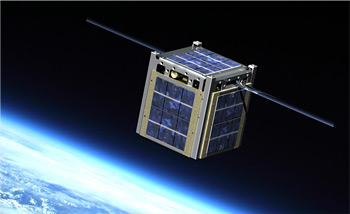
\includegraphics[width=0.8\linewidth]{./figs/cubesat_01}
			
		\begin{small}
			FONTE: \textit{NASA}\textsuperscript{\cite{NASA}}
		\end{small}		
	\end{figure}
		
	O \textit{CubeSat} Mauá, proposto no NSEE-IMT, é um equipamento do modelo 3U, sendo as unidades distribuídas em unidade de comunicação, unidade de controle de atitude e unidade de potência, como apresentado na Figura \ref{Fig_Est_Cubo}.
	
	\begin{figure}[th]
		\caption{ESTRUTURA DO CUBESAT PROPOSTA PELO NSEE-IMT}
		\label{Fig_Est_Cubo}
		\centering
		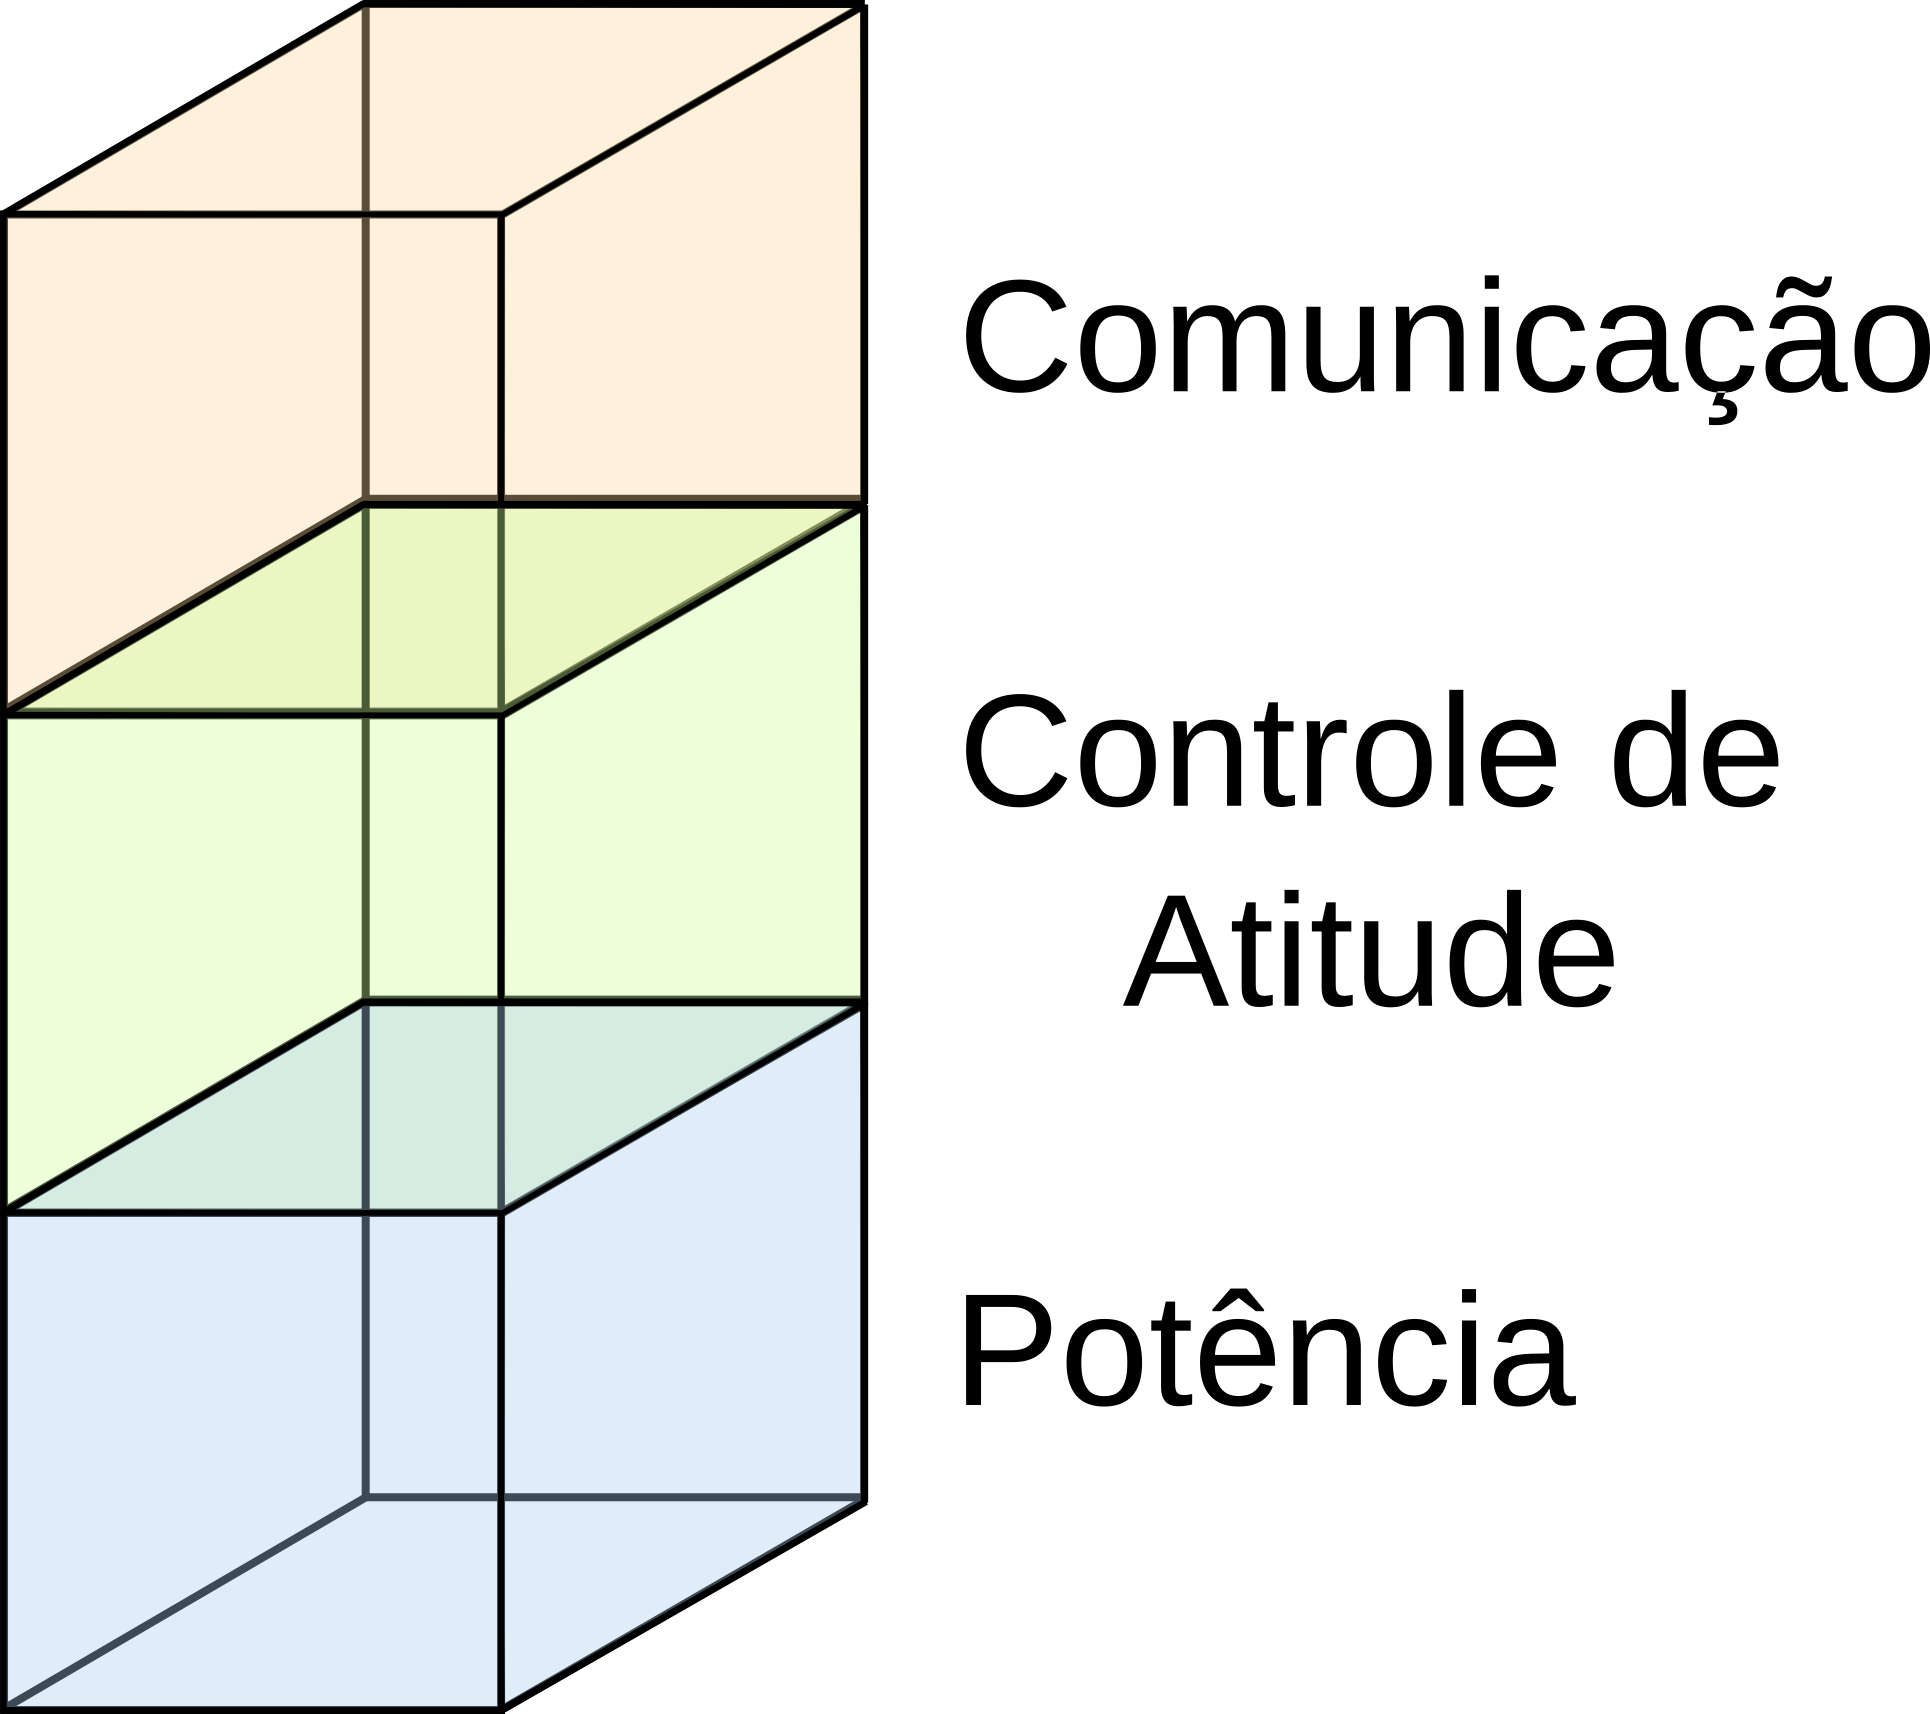
\includegraphics[width=0.4\linewidth]{./figs/cubesat_02}
			
		\begin{small}
			FONTE: Especificação do produto CubeSat\textsuperscript{\cite{Corsi}}
		\end{small}		
	\end{figure}
	\pagebreak

\section[Surgimento]{Surgimento} 

	O primeiro projeto de um \textit{CubeSat} foi proposto em 1.999 pelos professores Jordi Puig-Suari, da \textit{California Polytechnic State University}, e Bob Twiggs, da \textit{Stanford University}. O objetivo do projeto foi o de padronizar o \textit{design} de picosatélites, visando a redução de custos e de tempo de desenvolvimento, além de prover uma maior acessibilidade ao espaço e conseguir realizar lançamentos frequentes, o que é de inviável obtenção com os satélites de grande porte.\textsuperscript{\cite{CubeSat}}
	
	Já em 2.004, os \textit{CubeSats} podiam ser construídos por um custo estimado de \$65.000 a \$80.000. Esse custo, muito inferior comparado ao de satélites "convencionais", fez do \textit{CubeSat} uma opção viável para que escolas e universidades ao redor do mundo difundissem a tecnologia aplicada no segmento aeroespacial. Por conta desse custo relativamente baixo e da alta tecnologia inserida nesse contexto, um grande número de universidades, empresas e até mesmo instituições governamentais, passaram a desenvolver os \textit{CubeSats} para as mais variadas missões aeroespaciais.

\section[No Brasil]{No Brasil}

	Os projetos de picosatélites, nanosatélites e microsatélites se multiplicam a cada ano, não só no Brasil mas em todo o mundo. A \textit{Cal Poly} estima que atualmente o projeto \textit{CubeSat} conte com a colaboração internacional de mais de 100 universidades, colégios, empresas e governos.
	
	Atualmente vários projetos nessa área, de pequenos satélites para diversas áreas da pesquisa científica e tecnológica, estão em curso no Brasil e outros ainda em fase de discussão, dentre eles se destacam os projetos a seguir:
	\pagebreak
	
	\begin{itemize}
		\item \textbf{Tancredo 1}
		
			Picosatélite desenvolvido pelo grupo do professor Cândido Moura da Escola Tancredo Neves de Ubatuba, São Paulo. Primeiro satélite do Projeto UbatubaSat.\textsuperscript{\cite{UbatubaSat}}
			
		\item \textbf{AESP-14}		
		
			\textit{CubeSat} desenvolvido pelo grupo do Dr. Pedro Lacava, professor e coordenador do Curso de Engenharia Aeroespacial do Instituto Tecnológico de Aeronáutica (ITA).\textsuperscript{\cite{AESP14}}
			
		\item \textbf{NanoSatC-Br2}
		
			Nanosatélite em desenvolvimento pelo grupo coordenado pelo Dr. Nelson Schuch do Centro Regional Sul do INPE (CRS) e do Dr. Otávio Durão (INPE/SJC), em parceria com pesquisadores da Universidade Federal de Santa Maria (UFSM) do Rio Grande do Sul, em orbita desde 19/06/2.014.\textsuperscript{\cite{INPE}}

		\item \textbf{14-BISat}

			Nanosatélite científico em desenvolvimento pelo grupo liderado pelo professor Cedric Salotto, coordenador do Centro de Referência em Sistemas Embarcados e Aeroespaciais (CRSEA) do Instituto Federal Fluminense (IFF) da cidade de Campos dos Goytacazes (RJ), em parceria com a empresa \textit{Tekever S/A} e a Faculdade de Engenharia da Universidade do Porto (FEUP), Portugal. Este projeto faz parte da missão internacional QB50.\textsuperscript{\cite{IFF}}
			
		\item \textbf{ITASAT-1}	

			Nanosatélite tecnológico em desenvolvimento pelo grupo liderado pelo Major Eloi Fonseca, professor do Curso de Engenharia Aeroespacial do Instituto Tecnológico de Aeronáutica (ITA) em parceria com a Agência Espacial Brasileira (AEB), Instituto Nacional de Pesquisas Espaciais (INPE-SJC, INPE-CRN e INPE-SM), Universidade do Vale do Rio dos Sinos (UNISINOS), Universidade Federal do Rio Grande do Norte (UFRN) e Universidade Federal de Santa Maria (UFSM).\textsuperscript{\cite{ITASAT}}	
			
	\end{itemize}

\section[Características do meio]{Características do meio}
	
	Para o desenvolvimento do \textit{CubeSat} é de extrema importância ter conhecimento das condições de operação que o equipamento irá operar.
	
	Os \textit{CubeSats}, operam em órbita terrestre baixa (\textit{LEO - Low Earth Orbit}). A órbita \textit{LEO} é a órbita que se encontra abaixo de 2.000 km do nível do mar, os objetos que situam-se nela, geralmente, ficam entre 320 até 800 km da superfície terrestre, muito diferente dos satélites tradicionais que operam em órbita geoestacionária, cuja a distância é de 35.796 km em relação ao nível do mar.\textsuperscript{\cite{LEO}}\textsuperscript{\cite{GEO}}
	
	Satélites situados na órbita \textit{LEO} viajam em velocidades de aproximadamente 27.400 km/h ou 8 km/s, o que representa uma volta ao longo da Terra a cada 90 minutos. Já os satélites geoestacionários precisam ter uma velocidade que façam que eles acompanham sempre o mesmo ponto da Terra, por isso as velocidades deles são de aproximadamente 11.068 km/h ou 3 km/s. O planeta Terra tem uma velocidade de rotação de aproximadamente 1.669,8 km/h ou 0,5 km/s.\textsuperscript{\cite{LEO}}\textsuperscript{\cite{GEO}}
	
	Outras características de destaque para a órbita \textit{LEO} são as condições de temperatura, variando de -170 ºC a 123 ºC e de pressão variando de 10\textsuperscript{-4} Pa a 10\textsuperscript{-6} Pa.\textsuperscript{\cite{LEO}}
	
	Órbitas inferiores a esta não apresentam muita estabilidade e são alvos de arrastamento atmosférico, que é a força de fricção que atua sobre o foguete ou satélite, cuja principal causa é a fricção entre as moléculas do ar e a superfície do foguete ou satélite.\textsuperscript{\cite{NASA2}}
	
	\begin{figure}[th]
		\caption{PRINCIPAIS TIPOS DE ÓRBITAS}
		\label{Fig_Orbitas}
		\centering
		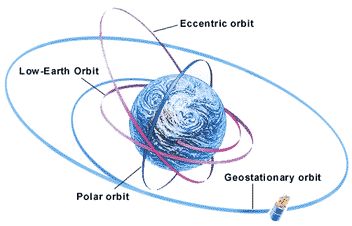
\includegraphics[width=0.65\linewidth]{./figs/cubesat_03}
			
		\begin{small}
			FONTE: Civil Air Patrol\textsuperscript{\cite{CAP}}
		\end{small}		
	\end{figure}
	
	A partir desse estudo preliminar fica mais fácil a compreensão e a definição dos critérios para a seleção dos componentes do projeto.	
	
\section[Bateria]{Bateria} \label{Sec_Bateria}
	
As baterias têm a função principal de armazenar carga e fornecer energia para todos os subsistemas do \textit{CubeSat}, incluindo os momentos no qual o equipamento estiver situado em regiões de sombras solares, por exemplo atrás do planeta Terra. Nessas regiões, não há incidência de luz solar portanto as fotocélulas não irão gerar energia no carregador da bateria. Dessa forma a bateria estará somente consumindo a energia armazenada até que o \textit{CubeSat} volte a ter incidência de luz solar para recomeçar o ciclo de carregamento, caso contrário o sistema será desligado e o equipamento virará apenas lixo espacial.	
	
	Algumas das premissas básicas de projeto para a definição da bateria estão relacionadas com o seu poder de armazenamento de carga e o seu dimensional reduzido. Essas baterias ficam alocadas no interior do \textit{CubeSat}, por isso a importância do dimensional reduzido, além disso não podem ser baterias com peso elevado, uma vez que a definição do projeto diz que os \textit{CubeSats} não podem ultrapassar 1,3 kg.
	
	Para a definição da bateria é necessário conhecer os tipos mais comuns de baterias encontradas no mercado, sendo elas de: níquel cádmio (NiCd), níquel-hidreto metálico (NiMh), íon-lítio (Li-Íon), íon-lítio polímero (Li-Íon polímero) e chumbo (Pb). Na Tabela \ref{Tab_Bateria} é possível analisar um comparativo dessas tecnologias, o que é de extrema importância para a definição da bateria correta. 
		
	\begin{table}[th]
		\caption{COMPARATIVO DAS TECNOLOGIAS UTILIZADAS}
		\label{Tab_Bateria}
		\begin{tabular}{p{3.5cm}|p{1.6cm}|p{1.6cm}|p{1.6cm}|p{2cm}|p{1.6cm}}
	 	& \textbf{NiCd} & \textbf{NiMh} & \textbf{Li-Íon} & \textbf{Li-Íon polímero} & \textbf{Pb} \\
	 	\hline
		\textbf{Densidade energética (Wh/kg)} & 45-80 & 60-120 & 110-160 & 100-130 & 30-50 \\
	 	\hline
	 	\textbf{Resistência interna (m$\Omega$)} & 100-200\textsuperscript{a} & 200-300\textsuperscript{a} & 150-250\textsuperscript{b} & 200-300\textsuperscript{b} & <100\textsuperscript{c} \\
	 	\hline
	 	\textbf{Ciclo de vida} & 1500 & 500-1000 & 500-1000 & 300-500 & 200-300 \\
		\hline
		\textbf{Tempo para carga rápida} & 1 hr & 2-4 hr & 2-4 hr & 2-4 hr & 8-16 hr \\
		\hline
		\textbf{Tolerância para sobrecarga} & Moderada & Baixa & Muito baixa & Baixa & Alta \\
		\hline
		\textbf{Auto-descarga mensal} & 20\% & 30\% & 10\% & 10\% & 5\% \\
		\hline
		\textbf{Tensão da célula (V)} & 1,25 & 1,25 & 3,6 & 3,6 & 2 \\
		\hline
		\textbf{Corrente de carga (In)} & 1,0 & 0,5 & 1,0 & 1,0 & 0,2 \\
		\hline
		\textbf{Temperatura de operação (ºC)} & -40 a 60 & -20 a 60 & -20 a 60 & 0 a 60 & -20 a 60 \\
		\hline
		\textbf{Manutenção (dias)} & 30-60 & 60-90 & --- & --- & 90-180 \\
		\hline
		\textbf{Comparação de custo \textit{pack} 7,2 V (dólar)} & 50,00 & 60,00 & 100,00 & 100,00 & 25,00 \\
		\hline
		\textbf{Custo por ciclo (dólar)} & 0,04 & 0,12 & 0,14 & 0,29 & 0,10 \\
		\hline 
		\end{tabular}
	\centering
	\begin{small}
	\vspace{3pt}
		FONTE: STA Eletrônica\textsuperscript{\cite{sta}}
	\end{small}
	
	\begin{footnotesize}
		NOTA: a: \textit{pack} 6V; b: \textit{pack} 7,2V; c: \textit{pack} 12V.
	\end{footnotesize}
	\end{table}

	Dentre os modelos analisados, as baterias de íon-lítio apresentam algumas características superiores aos demais modelos, como:
	\pagebreak
	
	\begin{itemize}
		\item Alta densidade energética;
		\item Alto ciclo de vida;
		\item Baixa auto-descarga mensal;
		\item Alta tensão da célula;
		\item Sem necessidade de manutenção;
		\item Amplo intervalo de temperatura de operação.
	\end{itemize}


\subsection[Princípio de funcionamento]{Princípio de funcionamento}

	
	As baterias de íon-lítio, têm esse nome devido ao seu princípio de funcionamento o qual consiste no movimento dos íons de lítio por meio de um solvente não aquoso.\textsuperscript{\cite{BraEsc}}	
	
	Na bateria de íon-lítio, o ânodo é feito de carbono enquanto o cátodo de algum óxido de metal que contenha lítio. Ambos os terminais ficam imersos a um eletrólito com um separador entre eles. Quando adicionada uma carga à esses terminais, os íons de lítio migram do ânodo para o cátodo, se os terminais são conectados a um carregador o processo ocorre de forma inversa,  ou seja, os íons de lítio partem do cátodo para o ânodo.\textsuperscript{\cite{sony}}
	
	Para haver essa movimentação dos íons de lítio, o que deixa a bateria com a característica de ser recarregável, nenhum dos terminais (ânodo ou cátodo) dessa bateria pode ser puramente do metal lítio.\textsuperscript{\cite{sony}}
	
	Na Figura \ref{Fig_PF_Bat}, pode ser visto o mecanismo de carga e descarga de uma bateria de íon-lítio.
	
	\begin{figure}[th]
		\caption{PRINCÍPIO DE FUNCIONAMENTO DA BATERIA DE ÍON-LÍTIO}
		\label{Fig_PF_Bat}
		\centering
		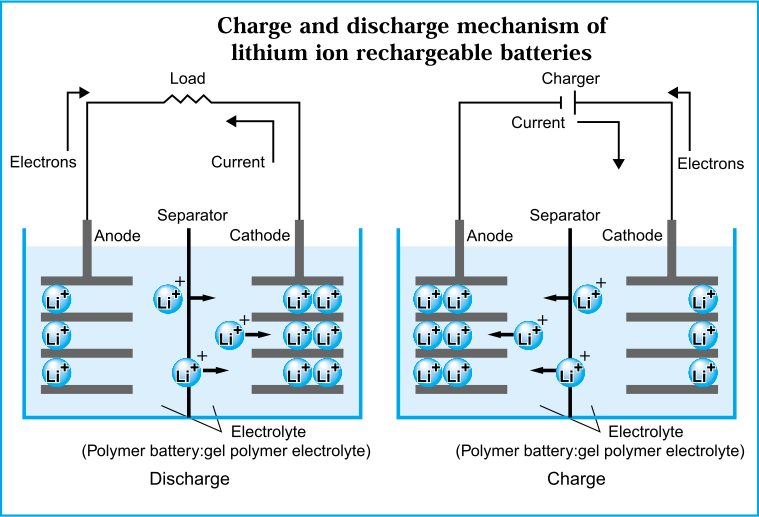
\includegraphics[width=0.6\linewidth]{./figs/funcionamento_bateria}
			
		\begin{small}
			FONTE: Sony Corporation\textsuperscript{\cite{sony}}
		\end{small}		
	\end{figure}
	\pagebreak

	O lítio (Li) é considerado o metal mais leve existente na Terra (desconsiderando os feitos em laboratório), por essa razão que as baterias de íon-lítio possuem baixo peso, o que é de fundamental importância para o projeto do \textit{CubeSat}. Por se tratar de um dos tipos de bateria mais comuns, sendo amplamente encontrado em \textit{smartphones} e \textit{notebooks}, acaba tendo um impacto positivo nos custos de aquisição das mesmas.\textsuperscript{\cite{TecMundo}}
	
\section[Fotocélulas]{Fotocélulas} \label{Cap_Cell}

	As fotocélulas são de fundamental importância para o sistema, uma vez que elas são as responsáveis pela captação da luz solar que irá gerar a energia necessária para o funcionamento do \textit{CubeSat}. É importante que elas possuam rendimento elevado, pois devido as condições impostas pela órbita \textit{LEO}, na qual o \textit{CubeSat} irá ficar um terço do período de translação em regiões de sombra, ou seja, estará sem a incidência direta de luz solar, conforme Figura \ref{Fig_Cone_Solar}.
	
	\begin{figure}[th]
		\caption{INCIDÊNCIA DE LUZ SOLAR}
		\label{Fig_Cone_Solar}
		\centering
		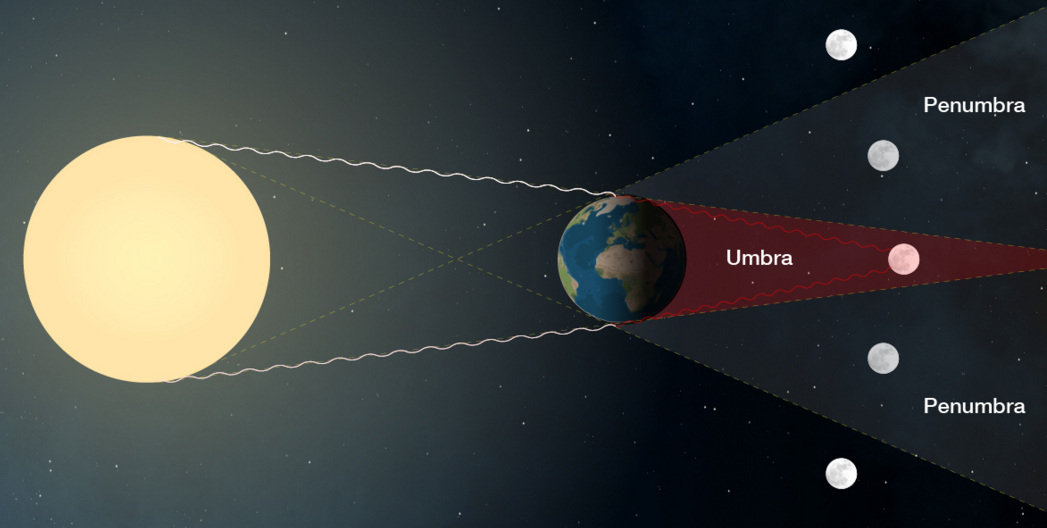
\includegraphics[width=0.7\linewidth]{./figs/cone_solar}
			
		\begin{small}
			FONTE: \textit{NASA}.\textsuperscript{\cite{NASA3}}
		\end{small}		
	\end{figure}
	
	Inicialmente as fotocélulas eram fabricadas a partir do Silício, na década de 1.960 essas células apresentavam aproximadamente 10\% de eficiência, atualmente essa eficiência chega próximo aos 20\%. No final da década de 1.980 começaram a ser produzidas fotocélulas de Arseneto de Gálio, as quais atingiram uma eficiência superior a 20\%, essa nova composição começou porque as fotocélulas de Silício chegaram a ser produzidas com Silício de alta pureza (99,999999\%). Após as primeiras células de Arseneto de Gálio foi adicionado a sua composição o Índio, obtendo ótimos resultados.\textsuperscript{\cite{Fatemi}}
	
	Nas fotocélulas de uma única junção, esse excesso de energia se converte em calor, ou seja, é uma perda de energia absorvida. A técnica de multijunções atenua o problema da perda de energia quando um fóton de energia maior do que a energia do semicondutor é absorvido. Nessas fotocélulas cada junção funciona como um filtro, ou seja, cada junção absorve uma parte do espectro de luz e deixa o restante passar para a próxima junção, dessa maneira o rendimento é muito melhor devido ao alto aproveitamento do espectro.\textsuperscript{\cite{Fatemi}}
	
	\begin{figure}[th]
		\caption{COMPARATIVO DOS MODELOS DAS FOTOCÉLULAS}
		\label{Fig_cells}
		\centering
		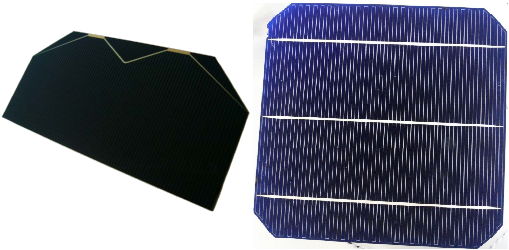
\includegraphics[width=0.7\linewidth]{./figs/cells}
			
		\begin{small}
			FONTE: Fotos editadas pelos autores.
		\end{small}		
	\end{figure}
	
	Na Figura \ref{Fig_cells}, é possível visualizar a diferença entre as tecnologias, no lado esquerdo está uma fotocélula com tecnologia aeroespacial ao lado de uma fotocélula com tecnologia industrial.
	
\subsection[Comparativo das tecnologias]{Comparativo das tecnologias}

	Devido as opções disponíveis de tecnologia foram realizados alguns estudos com o intuito de se obter qual seria o melhor tipo de fotocélula para o seguimento do projeto. A seguir serão comparados as principais métricas necessárias para uma fotocélula de aplicação espacial.
	
	\begin{figure}[th]
		\caption{COMPARATIVO DE EFICIÊNCIA DAS FOTOCÉLULAS}
		\label{Fig_cell_comp1}
		\centering
		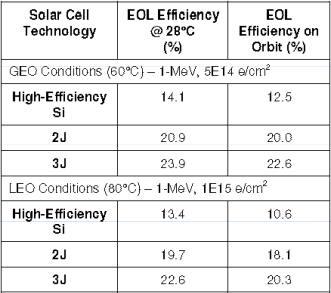
\includegraphics[width=0.55\linewidth]{./figs/cell_comp1}
			
		\begin{small}
			FONTE: \textit{Solar array trades between very high-efficiency multi-junction ans Si space solar cells}.\textsuperscript{\cite{Fatemi}}
		\end{small}
		
		\begin{footnotesize}
			NOTA: \textit{EOL} - \textit{End-of-life}.
		\end{footnotesize}
	\end{figure}
	
	Na Figura \ref{Fig_cell_comp1} é visível que as fotocélulas de tripla junção são mais eficientes e resistentes a radiação do que as demais tecnologias analisadas (Sílicio e dupla junção).
	
	\begin{figure}[th]
		\caption{COMPARATIVO DE POTÊNCIA DAS FOTOCÉLULAS}
		\label{Fig_cell_comp2}
		\centering
		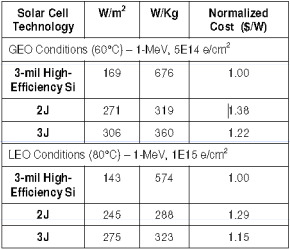
\includegraphics[width=0.6\linewidth]{./figs/cell_comp2}
			
		\begin{small}
			FONTE: \textit{Solar array trades between very high-efficiency multi-junction ans Si space solar cells}.\textsuperscript{\cite{Fatemi}}
		\end{small}
	\end{figure}	
	
	Já na Figura \ref{Fig_cell_comp2}, é realizado um comparativo da potência pela área e da potência pela massa. Nesse comparativo pode-se ver, novamente, que as fotocélulas de tripla função levam vantagem em relação as demais quando analisado a Potência (W) pela área (m\textsuperscript{2}), pois essa tecnologia permite um melhor aproveitamento do espectro de luz absorvido, conforme pode ser visto na Figura \ref{Fig_cell_mult}. 
	
	\begin{figure}[th]
		\caption{ESQUEMA DE UMA CÉLULA MULTIJUNÇÃO E SEU ESPECTRO}
		\label{Fig_cell_mult}
		\centering
		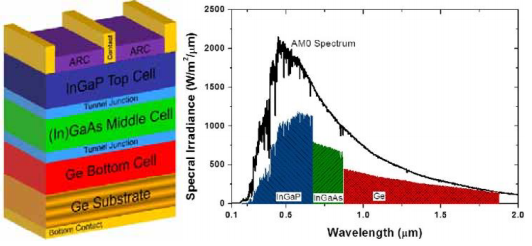
\includegraphics[width=.9\linewidth]{./figs/cell_mult}
			
		\begin{small}
			FONTE: \textit{Solar array trades between very high-efficiency multi-junction ans Si space solar cells}.\textsuperscript{\cite{Fatemi}}
		\end{small}		
	\end{figure}
	\pagebreak
	
	E por fim, quando o comparativo é em relação a massa das fotocélulas, a de Sílicio leva vantagem devido ao menor peso que possui comparada as demais, como visto na Figura \ref{Fig_cell_comp3}
	
	\begin{figure}[th]
		\caption{COMPARATIVO DE DIMENSÃO DAS FOTOCÉLULAS}
		\label{Fig_cell_comp3}
		\centering
		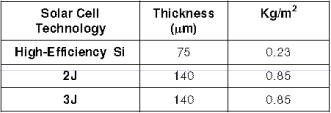
\includegraphics[width=0.6\linewidth]{./figs/cell_comp3}
			
		\begin{small}
			FONTE: \textit{Solar array trades between very high-efficiency multi-junction ans Si space solar cells}.\textsuperscript{\cite{Fatemi}}
		\end{small}		
	\end{figure}
	
	Com base nos comparativos apresentados nas Figuras \ref{Fig_cell_comp1}, \ref{Fig_cell_comp2} e \ref{Fig_cell_comp3}, foi definido que as fotocélulas de tripla junção seriam as mais adequadas para a continuidade do projeto.
	
\subsection[Princípio de funcionamento]{Princípio de funcionamento}

	As fotocélulas são um exemplo de aplicação prática do efeito fotoelétrico, descoberto por Heinrich Rudolf Hertz, em 1.887 e explicado por Albert Einstein, em 1.905.\textsuperscript{\cite{celula}}
	
	Quando uma grande quantidade de fótons é incidida em uma fotocélula a energia é absorvida. Essa absorção de energia permite que os átomos dos elementos que constituem a célula liberem elétrons, o espaço liberado é preenchido por outro elétron de uma camada inferior do semicondutor. Essa movimentação de elétrons, faz com que um dos lados da célula tenha uma concentração maior de elétrons, o que origina a diferença de potencial entre os lados, conforme pode ser visto na Figura \ref{Fig_PF_Cell}.\textsuperscript{\cite{celula2}}
	
	\begin{figure}[th]
		\caption{PRINCÍPIO DE FUNCIONAMENTO DE UMA FOTOCÉLULA}
		\label{Fig_PF_Cell}
		\centering
		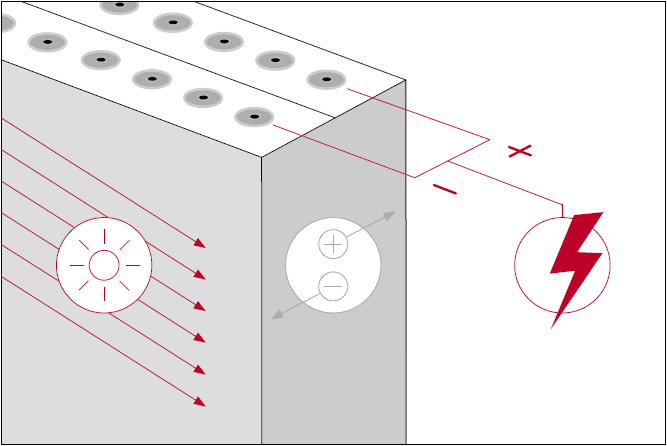
\includegraphics[width=0.6\linewidth]{./figs/fotocelula}
			
		\begin{small}
			FONTE: Sapa Solar\textsuperscript{\cite{celula2}}
		\end{small}		
	\end{figure}
	
\subsection[VIS Technology]{\textit{VIS Technology}}
	
	Inicialmente foi indicado pelo Engenheiro Rafael Corsi, do NSEE-IMT, o contato da empresa \textit{Vis Technology}, um empresa nacional, localizada em São Paulo, que desenvolve projetos com energias renováveis. Porém as fotocélulas utilizadas por eles são para aplicações industriais. Essas fotocélulas possuem um rendimento entre 10\% e 12\%, muito abaixo comparado ao rendimento com as próprias de aplicações aeroespaciais, além de terem um dimensional maior, conforme pode ser visualizado na Figura \ref{Fig_Cell_Vis}.
	
	\begin{figure}[th]
		\caption{FOTOCÉLULAS DA \textit{VIS TECHNOLOGY}}
		\label{Fig_Cell_Vis}
		\centering
		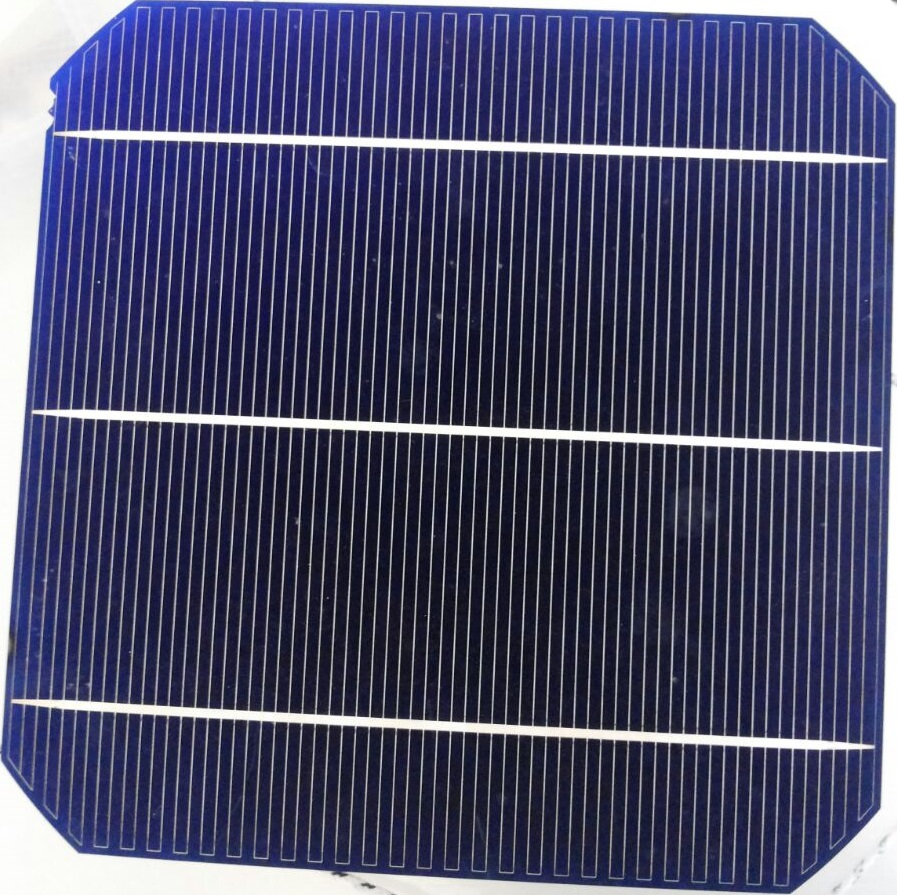
\includegraphics[width=0.6\linewidth]{./figs/cell_vis}
			
		\begin{small}
			FONTE: Foto tirada pelos autores.
		\end{small}		
	\end{figure}
	
	Mesmo sabendo dessas limitações, foram obtidas algumas amostras. Essas amostras serviram para um primeiro contato com essa tecnologia, conseguindo realizar alguns ensaios a fim de se obter uma familiaridade maior com o componente.
	
	Após uma breve familiarização com as fotocélulas, foram analisados diversos projetos de \textit{CubeSats} e identificados os principais fornecedores de fotocélulas (\textit{SpectroLab}, \textit{Emcore} e \textit{AzurSpace Solar}) para aplicações aeroespaciais.
	
	Foi realizado um estudo apurado dos principais tipos de fotocélulas disponíveis nos portfólios desses fornecedores, visando identificar os modelos que se melhor ajustavam no desenvolvimento do \textit{CubeSat}.
	
\subsection[SpectroLab]{\textit{SpectroLab}}
	
	A \textit{SpectroLab}, empresa subsidiária da \textit{The Boeing Company}, é a fabricante líder mundial de células solares de multi-junção de alta eficiência e de painéis solares. A empresa é sediada nos Estados Unidos, mais especificamente em Los Angeles, Califórnia.\textsuperscript{\cite{SpectroLab}}
	
	\begin{table}[th]
	\caption{COMPARATIVO DAS FOTOCÉLULAS DA \textit{SPECTROLAB}}
	\label{Tab_Spectro_Comp}
	\begin{tabular}{p{2.5cm}|p{3.1cm}|p{3.1cm}|p{3.1cm}|p{3.1cm}}
		\textbf{Modelo} & \textit{\textbf{PV UTJ Cell}} & \textit{\textbf{PV XTJ Cell}} & \textit{\textbf{PV NM TASC ITJ}} & \textit{\textbf{PV ITJ Cell}} \\
		\hline
		\textbf{Rendimento} & 28,3\% & 29,5\% & 24\% a 30\% & 26,8\% \\
		\hline
		\textbf{Material} & GaInP2/GaAs/Ge & GaInP2/GaAs/Ge & GaInP2/GaAs/Ge & GaInP2/GaAs/Ge\\
		\hline
		\textbf{Tensão} & 2,660 V & 2,633 V & 2,520 V & 2,565 V\\
		\hline
		\textbf{Corrente} & 454 mA & 472 mA & 31 mA & 441 mA\\
		\hline
		\textbf{Dimensional} & 26,62 cm\textsuperscript{2} & 26,62 cm\textsuperscript{2} & 2,277 cm\textsuperscript{2} & 31 cm\textsuperscript{2}\\
		\hline
		\textbf{Peso} & 84 mg/cm\textsuperscript{2} & 84 mg/cm\textsuperscript{2} & 0,234 g & 84 mg/cm\textsuperscript{2}\\
	\end{tabular}
	
	\begin{small}
	\vspace{3pt}
		FONTE: Elaborada pelos autores através de informações coletadas nos \textit{datasheets} dos produtos.
	\end{small}
	\begin{footnotesize}
		NOTA: Condições de teste: \textit{AM} 0, \textit{WRC} = 135,3 mW/cm\textsuperscript{2}, T = 28ºC.
	\end{footnotesize}
	\end{table}

	Avaliando os dados da Tabela \ref{Tab_Spectro_Comp}, os modelos \textit{PV UTJ Cell} e \textit{PV XTJ Cell}, foram os mais indicados para a aplicação, devido ao alto rendimento (superior a 28\%) apresentado
	
	\begin{figure}[th]
		\caption{MODELO DE FOTOCÉLULA DA \textit{SPECTROLAB}}
		\label{Fig_Cell_Spectro}
		\centering
		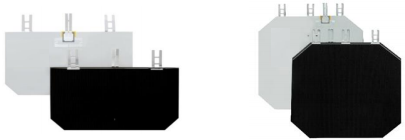
\includegraphics[width=1.0\linewidth]{./figs/UTJ}
			
		\begin{small}
			FONTE: \textit{SpectroLab}\textsuperscript{\cite{SpectroLab2}}
		\end{small}		
	\end{figure}

\subsection[Emcore]{\textit{Emcore}}

	Em dezembro de 2014, a \textit{Emcore} foi comprada pela \textit{SolAero Technologies}, que é uma das fabricantes líderes mundial de alta eficiência, células solares e painéis solares para aplicações espaciais. Assim como a \textit{SpectroLab}, está sediada nos Estados Unidos, porém no município de Albuquerque, Novo México.\textsuperscript{\cite{Emcore}}\textsuperscript{\cite{Emcore2}}
	
	\begin{table}[th] 
	\caption{COMPARATIVO DAS FOTOCÉLULAS DA \textit{EMCORE}}
	\label{Tab_Emcore_Comp}
	\begin{tabular}{p{2.5cm}|p{3.1cm}|p{3.1cm}|p{3.1cm}|p{3.1cm}}
		\textbf{Modelo} & \textit{\textbf{ATJ PV Cell}} & \textit{\textbf{BTJ PV Cell}} & \textit{\textbf{BTJM PV Cell}} & \textit{\textbf{ZTJ PV Cell}} \\
		\hline
		\textbf{Rendimento} & 27,5\% & 28,5\% & 28\% & 29,5\% \\
		\hline
		\textbf{Material} & GaInP/GaAs/Ge & GaInP/GaAs/Ge & GaInP/GaAs/Ge & GaInP/GaAs/Ge\\
		\hline
		\textbf{Tensão} & 2,60 V & 2,70 V & 2,69 V & 2,73 V\\
		\hline
		\textbf{Corrente} & 454 mA & 455 mA & 454 mA & 467 mA\\
		\hline
		\textbf{Dimensional} & 26,6 cm\textsuperscript{2} & 26,6 cm\textsuperscript{2} & 26,6 cm\textsuperscript{2} & 26,6 cm\textsuperscript{2}\\
		\hline
		\textbf{Peso} & 84 mg/cm\textsuperscript{2} & 84 mg/cm\textsuperscript{2} & 84 mg/cm\textsuperscript{2} & 84 mg/cm\textsuperscript{2}\\
	\end{tabular}
	
	\begin{small}
	\vspace{3pt}
		FONTE: Elaborada pelos autores através de informações coletadas nos \textit{datasheets} dos produtos.
	\end{small}
	\begin{footnotesize}
		NOTA: Condições de teste: \textit{AM} 0, \textit{WRC} = 135,3 mW/cm\textsuperscript{2}, T = 28ºC.
	\end{footnotesize}
	\end{table}
	\pagebreak
	Avaliando os dados da Tabela \ref{Tab_Emcore_Comp}, os modelos \textit{BTJ PV Cell}, \textit{BTJM PV Cell} e \textit{ZTJ PV Cell}, foram os mais indicados para a aplicação, devido ao alto rendimento (superior a 28\%) apresentado.
	
	\begin{figure}[th]
		\caption{MODELO DE FOTOCÉLULA DA \textit{EMCORE}}
		\label{Fig_Cell_Emcore}
		\centering
		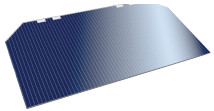
\includegraphics[width=0.5\linewidth]{./figs/ZTJ}
			
		\begin{small}
			FONTE: \textit{SolAero Technologies}\textsuperscript{\cite{Emcore3}}
		\end{small}		
	\end{figure}

\subsection[AzurSpace]{\textit{AzurSpace}}

	A \textit{AzurSpace} é a líder européia no desenvolvimento e produção de células solares multi-junção para aplicações espaciais e terrestres, com quase 50 anos de experiência no mercado. A empresa localiza-se em Heilbronn, cidade em Baden-Württemberg, Alemanha.\textsuperscript{\cite{AzurSpace}}
	
	\begin{table}[th]
	\caption{COMPARATIVO DAS FOTOCÉLULAS DA \textit{AZURSPACE}}
	\label{Tab_Azur_Comp}
	\begin{tabular}{p{2.5cm}|p{3.1cm}|p{3.1cm}|p{3.1cm}|p{3.1cm}}
		\textbf{Modelo} & \textit{\textbf{3G30C}} & \textit{\textbf{3G30C-Large}} & \textit{\textbf{3G30C-Large-120x60}} & \textit{\textbf{3G28C}} \\
		\hline
		\textbf{Rendimento} & 30\% & 30\% & 30\% & 28\% \\
		\hline
		\textbf{Material} & GaInP/GaAs/Ge & GaInP/GaAs/Ge & GaInP/GaAs/Ge & GaInP/GaAs/Ge\\
		\hline
		\textbf{Tensão} & 2,700 V & 2,700 V & 2,700 V & 2,667 V\\
		\hline
		\textbf{Corrente} & 520,2 mA & 1041 mA & 1186 mA & 506 mA\\
		\hline
		\textbf{Dimensional} & 30,18 cm\textsuperscript{2} & 60,36 cm\textsuperscript{2} & 68,76 cm\textsuperscript{2} & 30,18 cm\textsuperscript{2}\\
		\hline
		\textbf{Peso} & 86 mg/cm\textsuperscript{2} & 114 mg/cm\textsuperscript{2} & 130 mg/cm\textsuperscript{2} & 86 mg/cm\textsuperscript{2}\\
	\end{tabular}
	
	\begin{small}
	\vspace{3pt}
		FONTE: Elaborada pelos autores através de informações coletadas nos \textit{datasheets} dos produtos.
	\end{small}
	\begin{footnotesize}
		NOTA: Condições de teste: \textit{AM} 0, \textit{WRC} = 1367 W/m\textsuperscript{2}, T = 28 ºC.
	\end{footnotesize}
	\end{table}	
	
	Avaliando os dados da Tabela \ref{Tab_Azur_Comp}, os modelos \textit{30G28C} e \textit{30G30C}, foram os mais indicados para a aplicação, devido ao alto rendimento (superior a 28\%) apresentado. Os demais modelos não atenderam o dimensionamento adequado para o projeto.
	
	\begin{figure}[th]
		\caption{MODELO DE FOTOCÉLULA DA \textit{AZURSPACE}}
		\label{Fig_Cell_Azur}
		\centering
		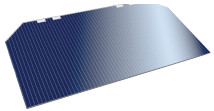
\includegraphics[width=0.5\linewidth]{./figs/ZTJ}
			
		\begin{small}
			FONTE: \textit{AzurSpace}\textsuperscript{\cite{AzurSpace2}}
		\end{small}		
	\end{figure}

\section[Componentes passivos]{Componentes passivos}\label{Cap_Passivo}

	Os componentes passivos, são os componentes eletrônicos que não aumentam a intensidade da tensão ou da corrente de um circuito eletrônico, ou seja, são os resistores, indutores, capacitores e memristores. No desenvolvimento do projeto não foram utilizados os memristores.\textsuperscript{\cite{Passivo}}
	
	Resistores são componentes utilizados para controlar a intensidade da corrente elétrica que passa no circuito. Capacitores são componentes que armazenam e liberam cargas elétricas por meio da tensão elétrica. Indutor são componentes que utilizam o magnetismo para armazenar e liberar cargas por meio da corrente elétrica.

	É de extrema importância que os componentes passivos atendam algumas premissas para a utilização no projeto. Esses componentes precisam possuir uma grande faixa de temperatura de operação, conforme ilustrado na Figura \ref{Fig_Range_Temp}, uma certa tolerância a radiação e um dimensional pequeno (\textit{SMD}).
	
	\begin{figure}[th]
		\caption{VARIAÇÃO DE TEMPERATURA E ALTITUDE}
		\label{Fig_Range_Temp}
		\centering
		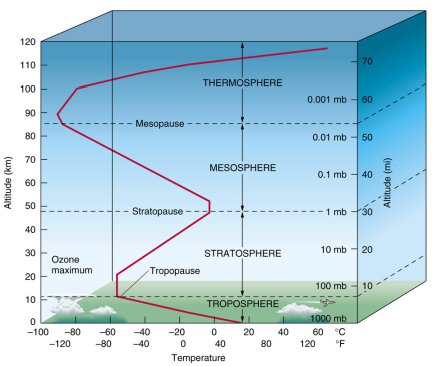
\includegraphics[width=0.8\linewidth]{./figs/orbita_temp}
			
		\begin{small}
			FONTE: \textit{SwissCube}\textsuperscript{\cite{SwissCube}}
		\end{small}		
	\end{figure}
	\pagebreak
	
	Os capacitores, devido as baixas pressões encontradas no espaço, não podem ser do modelo eletrolítico, ou seja, precisam ser de: ceramica, tântalo, poliester ou polipropileno. Os capacitores cerâmicos geralmente são de 0,5 pF até 470 nF com tensão de isolação de 25 V ou 50 V. Para esses capacitores tomou-se o cuidado de selecionar os capacitores com baixo \textit{ESR} e com o coeficiente de temperatura X7R, devido a sua grande faixa de temperatura de operação, conforme indicado na Figura \ref{Fig_Cap}.\textsuperscript{\cite{x7r}}
	
	\begin{figure}[th]
		\caption{COEFICIENTES DE TEMPERATURA DOS CAPACITORES CERÂMICOS}
		\label{Fig_Cap}
		\centering
		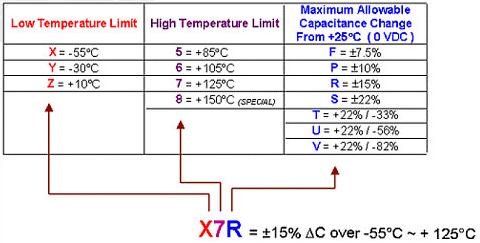
\includegraphics[width=0.8\linewidth]{./figs/x7r}
			
		\begin{small}
			FONTE: PY2BBS\textsuperscript{\cite{x7r}}
		\end{small}		
	\end{figure}	
	\pagebreak
	
	O \textit{ESR}, resistência equivalente em série, significa que um capacitor possui uma resistência interna que com o passar do tempo aumenta ao ponto de ser maior que a reatância capacitiva do mesmo.\textsuperscript{\cite{esr}}.
		
	Além dessa característica, os capacitores X7R apresentam um bom comportamento com a variação de temperatura, comparado com os capacitores Y5V (outro modelo amplamente encontrado no mercado), conforme pode ser visto na Figura \ref{Fig_Cap_Temp}.
	
	\begin{figure}[th]
		\caption{VARIAÇÃO DA CAPACITÂNCIA EM FUNÇÃO DA TEMPERATURA}
		\label{Fig_Cap_Temp}
		\centering
		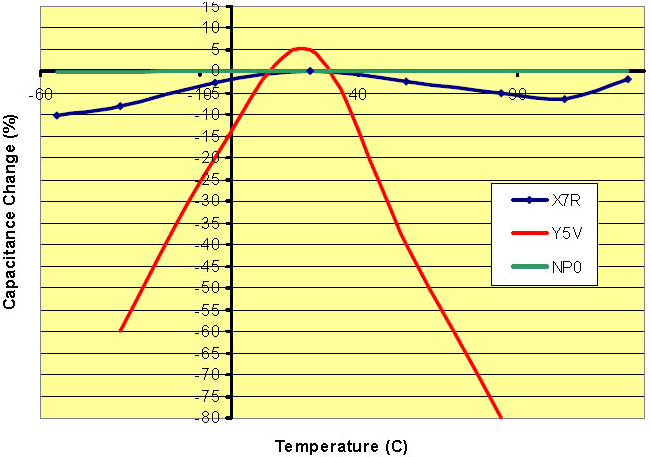
\includegraphics[width=0.8\linewidth]{./figs/y5v}
			
		\begin{small}
			FONTE: Johanson Dielectrics\textsuperscript{\cite{y5v}}
		\end{small}		
	\end{figure}

	Já os capacitores de tântalo apresentam valores de 0,22 pF até 100 $\mu$F, esse tipo de capacitor possui baixa corrente de fuga e baixas perdas, além de uma vida útil maior comparado aos eletrolíticos.\textsuperscript{\cite{x7r}}

\section[Semicondutores]{Semicondutores}

Elementos semicondutores são os elementos químicos que possuem na sua camada de valência quatro elétrons. A condutividade desses elementos depende da temperatura na qual estão submetidos. Os principais elementos utilizados na construção de semicondutores, por exemplo diodos, transistores e circuitos integrados, são o silício e o germânio. A grande maioria dos semicondutores são construídos com silício, uma vez que o germânio é extremamente sensível a variações de temperatura.\textsuperscript{\cite{semicondutores}}
	
	Os semicondutores formam bandas de energia, como a banda de condução e a banda de valência, essas bandas são separadas por lacunas. A banda de condução vai estar vazia e a banda de valência totalmente preenchida quando estiver com uma temperatura de 0K (-273,15 ºC ou zero absoluto), como pode ser visto na Figura \ref{Fig_bandas}.\textsuperscript{\cite{semicondutores2}}\textsuperscript{\cite{kelvin}}
	
	\begin{figure}[th]
		\caption{BANDAS DE ENERGIA DE UM SEMICONDUTOR}
		\label{Fig_bandas}
		\centering
		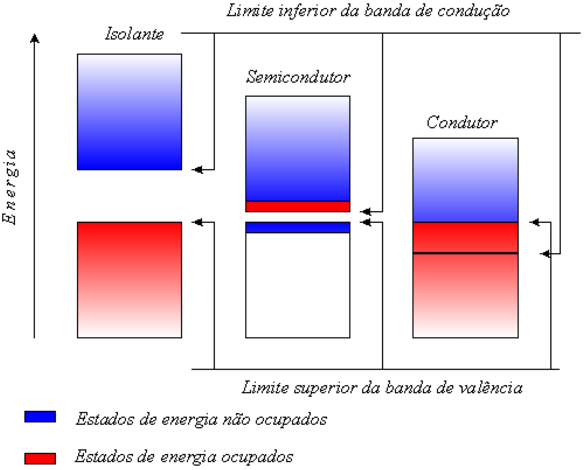
\includegraphics[width=0.8\linewidth]{./figs/banda}
			
		\begin{small}
			FONTE: Professor Dr. Eduardo Fontana\textsuperscript{\cite{doutor}}
		\end{small}		
	\end{figure}

	Com a variação de temperatura, alguns dos elétrons migram da banda de valência para a a banda de condução, devido ao ganho de energia no elétron.

	Em condições normais, os semicondutores possuem uma baixa condutividade, para contornar esse problema são dopadas impurezas. Essas impurezas podem ser do tipo doadora ou aceitadoras. O semicondutor dopado com uma impureza doadora é denominado do tipo N. Já os dopados com a impureza aceitadora é denominado do tipo P.\textsuperscript{\cite{semicondutores2}}
	
\subsection[Carregador de bateria]{Carregador de bateria}

	Os carregadores de bateria basicamente consistem em uma fonte de corrente que gera uma corrente contrária ao da célula da bateria, como visualizado na Figura \ref{Fig_PF_Bat}. Como a resistência interna de uma bateria é baixa, é necessário ter um limitador de corrente para manter a carga com uma corrente segura, conforme Figura \ref{Fig_Carregador}.\textsuperscript{\cite{carregador}}
	
	\begin{figure}[th]
		\caption{CARREGADOR SIMPLES DE BATERIA}
		\label{Fig_Carregador}
		\centering
		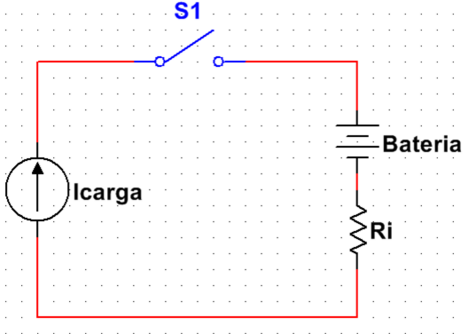
\includegraphics[width=0.5\linewidth]{./figs/carregador}
			
		\begin{small}
			FONTE: Elaborado pelos autores.
		\end{small}		
	\end{figure}
	\pagebreak
	
	Alguns carregadores são limitados de acordo com a indicação do fabricante da bateria, que diz qual a corrente que deve passar pela célula para realizar o carregamento. Também é necessário tomar o devido cuidado com correntes excessivas durante a recarga, a circulação da corrente além de repor a energia nas células da bateria, também gera calor através de efeito Joule, devido a dissipação de calor na resistência interna da mesma. Aquecimentos excessivos podem resultar em consequências drásticas para a integridade da bateria, gerando possíveis danos no eletrodos ou na própria composição química do eletrólito, podendo em alguns casos até ocorrer a explosão da bateria devido a formação de gases sob pressão.\textsuperscript{\cite{carregador}}
	
	Atualmente existem diversos carregadores de baterias que são chamados de carregadores inteligentes, esses carregadores recebem esse nome devido a sua capacidade de gerenciamento do carregamento da bateria.
	
	Alguns recursos são utilizados para se obter uma maior eficiência e também uma prolongação da vida útil da bateria. Um desses recursos é a utilização de um regime de corrente constante, ou seja, em uma célula totalmente descarregada a diferença de potencial nos seus terminais é baixa, dessa forma ao aplicar uma tensão no carregador a diferença entre essas tensões é elevada, o que leva a circulação de uma corrente inicial elevada, como pode ser exemplificado na Figura \ref{Fig_Temp_Carg}.\textsuperscript{\cite{carregador}}
	
	\begin{figure}[th]
		\caption{CURVA DE CARREGAMENTO INTELIGENTE}
		\label{Fig_Temp_Carg}
		\centering
		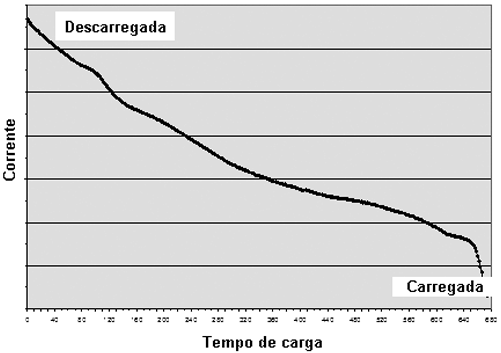
\includegraphics[width=0.67\linewidth]{./figs/temp_carg}
			
		\begin{small}
			FONTE: \textit{Marine service}\textsuperscript{\cite{marine}}
		\end{small}	
	\end{figure}
	\pagebreak

	À medida que a bateria vai carregando, a tensão entre os seus terminais vai se elevando de modo a se contrapor à tensão do carregador, dessa forma a corrente de carga na bateria diminui de forma gradual até que no final do processo de carga ela seja pequena e não linear.\textsuperscript{\cite{carregador}}
	
	Outro recurso disponível em carregadores inteligentes é o monitoramento da carga, da temperatura e das demais características importantes da bateria. Esses recursos são desde a adoção de regimes especiais de tempo de carga até a monitoração da tensão.

	A corrente varia com o tempo no processo de carga completa.	Dessa forma, o carregamento de uma bateria de íon-lítio deve ser feita em três etapas:
	
	\begin{enumerate}
		\item Carga lenta, carga feita com a corrente constante e tensão variável;
		\item Carga rápida, carga com tensão constante e corrente variável;
		\item Tensão constante e corrente constante.\textsuperscript{\cite{marine}}
	\end{enumerate}
	
	A carga lenta irá ocorrer quando a tensão da bateria estiver menor do que 2,5 V. As bateria de íon-lítio, por não apresentar efeito memória, podem ser recarregadas antes de haver uma descarga total da mesma, por tanto, em alguns casos o processo de carga lenta não é empregado nesse tipo de bateria.\textsuperscript{\cite{carregador}}
	
	Já o processo de carga rápida é a fase mais importante do processo, uma corrente constate irá carregar a bateria até ela atingir o seu nível máximo de carga. O circuito do carregador mede continuamente a corrente de sensoriamento (corrente em um resistor sensor ligado em série) ajustando o ciclo ativo do \textit{PWM} com o microcontrolador. Quando a tensão da bateria chega no seu valor máximo, o carregador passa a operar no modo de carga com tensão constante.\textsuperscript{\cite{carregador}}
	
	No modo de tensão constante, o circuito passa a operar como uma fonte de tensão, nesse momento a resistência interna da bateria começa a cair, o que exige uma compensação para manter a corrente baixa. Quando a bateria estiver completamente carregada, a maior parte da energia é convertida em calor.\textsuperscript{\cite{carregador}}

	Alguns métodos permitem determinar quando uma bateria está completamente carregada. Esses métodos são:
	
	\begin{itemize}
		\item Durante o processo de carga com tensão constante, quando a corrente cai a bateria se encontra completamente carregada;
		\item Determinar a temperatura da bateria de modo a se determinar quando começa a ocorrer o sobreaquecimento;
		\item Usar um método de temporização seguro. Quanto mais o tempo passar de um valor considerado ideal para a carga, a bateria poderá ser considerada completamente recarregada.
	\end{itemize}

\subsection[Conversores CC-CC]{Conversores CC-CC}

	Os conversores CC-CC (corrente contínua - corrente contínua) são circuitos eletrônicos que convertem as amplitudes de tensão e corrente contínua em outra amplitude. Essa conversão é realizada graças a semicondutores de potência operando como interruptores, além dos elementos passivos que formam o conjunto.\textsuperscript{\cite{semicondutores3}}
	
	Os principais tipos de conversores CC-CC são:
	
	\begin{minipage}{7cm}
		\begin{itemize}
			\item	\textit{Buck}
			\item	\textit{Boost}
			\item	\textit{Buck-boost}
			\item	Inversores
			\item	\textit{Forward}
			\item	\textit{Flyback}
	\end{itemize}
	\end{minipage}
	\begin{minipage}{7cm}
		\begin{itemize}
			\item	\textit{Push-pull}
			\item	\textit{Half bridge}
			\item	\textit{Full bridge}
			\item	\textit{Ćuk}
			\item	\textit{SEPIC}
		\end{itemize}
	\end{minipage}

	Para o projeto foram utilizados somente conversores dos tipos \textit{Buck} e \textit{Boost}. Esses dois tipos de conversores são conhecidos como conversores CC-CC diretos, pois neles existe a transferência direta da potência de entrada para a saída do conversor.
	
\subsection[Conversor Buck]{Conversor \textit{Buck}}

	O conversor \textit{Buck}, também conhecido como \textit{step-down}, é um conversor abaixador de tensão. Sua entrada é baseada em tensão e a saída em corrente, conforme pode ser visto na Figura \ref{Fig_buck}.\textsuperscript{\cite{inep}}
	
 	\begin{figure}[th]
		\caption{CONVERSOR \textit{BUCK}}
		\label{Fig_buck}
		\centering
		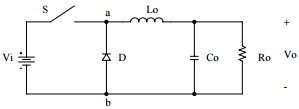
\includegraphics[width=0.75\linewidth]{./figs/buck}
			
		\begin{small}
			FONTE: INEP/EEL\textsuperscript{\cite{inep}}
		\end{small}		
	\end{figure}

	O princípio de funcionamento do conversor é relativamente simples. Quando a chave (S) está em modo de condução, a corrente flui pelo indutor (L\textsubscript{o}) e pela saída do circuito. A tensão de entrada (V\textsubscript{i}) fornece a energia para a saída do circuito e para a magnetização do indutor (L\textsubscript{o}).
	
	No instante da abertura da chave (S) o diodo (D) entra em condução, a energia do indutor (L\textsubscript{o}) é transferida para a carga (R\textsubscript{o}), ou seja, o indutor (L\textsubscript{o}) é desmagnetizado.
	
	Esse tipo de conversor tem três possíveis modos de operação:
	
	\begin{itemize} 
		\item[\textbf{1º}] Condução contínua - sem anulaçao da corrente no indutor (L\textsubscript{o}) durante o período de comutação;
		\item[\textbf{2º}] Condução descontínua - com anulação da corrente no indutor (L\textsubscript{o}) a cada período de comutação;
		\item[\textbf{3º}] Condução crítica - a corrente no indutor (L\textsubscript{o}) fica no limiar de se anular a cada período de comutação.
	\end{itemize}
	
	O conversor \textit{Buck} tem a capacidade de diminuir a tensão na saída, mantendo a boa qualidade da corrente de saída. A corrente de entrada é descontínua, uma vez que o conversor precisa fazer o chaveamento para que o sistema possa funcionar perfeitamente.\textsuperscript{\cite{inep}}
	
\subsection[Conversor Boost]{Conversor \textit{Boost}}

	O conversor \textit{Boost}, também conhecido como \textit{step-up}, é um conversor elevador de tensão. Ao contrário do conversor \textit{Buck}, sua entrada é baseada em corrente e a saída em tensão, conforme pode ser visto na Figura \ref{Fig_boost}.\textsuperscript{\cite{inep}}

 	\begin{figure}[th]
		\caption{CONVERSOR \textit{BOOST}}
		\label{Fig_boost}
		\centering
		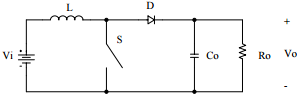
\includegraphics[width=0.75\linewidth]{./figs/boost}
			
		\begin{small}
			FONTE: INEP/EEL\textsuperscript{\cite{inep}}
		\end{small}		
	\end{figure}
	\pagebreak
	
	Seu princípio de funcionamento é, relativamente, similar ao do conversor \textit{Buck}. Quando a chave (S) está conduzindo, o indutor (L) é magnetizado, dessa forma a corrente flui somente entre a fonte (V\textsubscript{i}), o indutor (L) e a chave (S).
	
	Porém quando a chave (S) está aberta, o diodo (D) entra em condução, a fonte (V\textsubscript{i})e o indutor (L) fornecem energia à saída do circuito, aumentando a tensão na carga (R\textsubscript{o}).
	
	De forma resumida, o conversor \textit{Boost} pode apenas aumentar a tensão na saída do circuito, além de possuir uma boa qualidade da corrente de entrada. Porém possui uma corrente de saída descontínua, originado pelo chaveamento do que o circuito realiza para o seu funcionamento.\textsuperscript{\cite{inep}}
	
	Nesse capítulo foram apresentados os conceitos básicos do desenvolvimento de um \textit{CubeSat}, explicando o que é o \textit{CubeSat}, o meio no qual o equipamento irá operar e detalhando os principais componentes necessários para sua construção, assim como seus princípios de funcionamento. No capítulo a seguir, será abordado a seleção dos componentes assim como o método de trabalho realizado para realizar a construção da lista de componentes do projeto.


% ----------------------------------------------------------
% Materiais e Método
% ----------------------------------------------------------
\chapter[Materiais e método]{Materiais e método}

	Após a realização dos estudos apresentados no Capítulo \ref{Cap_Teorico}, a seleção dos materiais e dos métodos utilizados para o desenvolvimento do projeto se tornam mais amigáveis. 
	
	Essa seleção deve atender da melhor maneira possível os parâmetros levantados anteriormente, sendo bem fundamentada na teoria evitando surpresas no seu funcionamento. Lembrando que após o lançamento do \textit{CubeSat} não será possível nenhuma alteração e/ou correção de \textit{hardware}, sendo possível somente alguns ajustes de configuração de \textit{software}, como por exemplo alteração de parâmetros e de prioridades de tarefas.
	
% ----------------------------------------------------------
% Etapas
% ----------------------------------------------------------
\section[Topologia]{Topologia}

	A topologia do circuito foi o passo inicial para o desenvolvimento do Sistema de Gerenciamento de Energia para \textit{CubeSats}, onde foi definido através de um diagrama de blocos como funcionaria o circuito do projeto proposto.
	
	Diagrama de blocos é uma representação gráfica do modelo de um sistema e/ou processo complexo. É uma ferramenta extremamente difundida, utilizada como meio de referência para que pessoas não familiarizadas com o objeto de estudo, possam ter uma compreensão geral do projeto em questão.\textsuperscript{\cite{Diag_Blocos}}	
		
	Na Figura \ref{Fig_Diag_Blocos_Final}, pode ser visualizado o resultado final do diagrama de blocos utilizado no projeto.
	
	\begin{figure}[th]
		\caption{DIAGRAMA DE BLOCOS}
		\label{Fig_Diag_Blocos_Final}
		\centering
		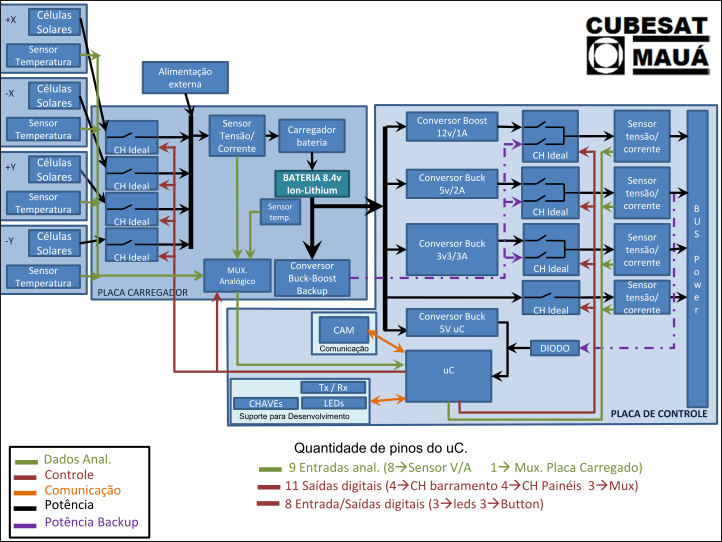
\includegraphics[width=1.0\linewidth]{./figs/diag_blocos}
			
		\begin{small}
			FONTE: Elaborado pelos autores.
		\end{small}		
	\end{figure}
	\pagebreak
	
	A definição do diagrama de blocos do Sistema de Gerenciamento de Energia para \textit{CubeSats} foi o passo inicial para o desenvolvimento do projeto, pois todo o estudo posterior foi realizado baseado no funcionamento do circuito pensado.

	Para atingir o nível de detalhe exibido no diagrama de blocos da Figura \ref{Fig_Diag_Blocos_Final}, diversas horas de estudos foram dedicadas, sendo essas horas distribuídas entre os estudos e através de diversos \textit{brainstorms} realizados pelo grupo.
	
	Na Figura \ref{Fig_Diag_Blocos_Inicial}, pode ser visualizado a ideia embrionária do diagrama de blocos pensado para o desenvolvimento do projeto.
		
	\begin{figure}[th]
		\caption{VERSÃO INICIAL DO DIAGRAMA DE BLOCOS}
		\label{Fig_Diag_Blocos_Inicial}
		\centering
		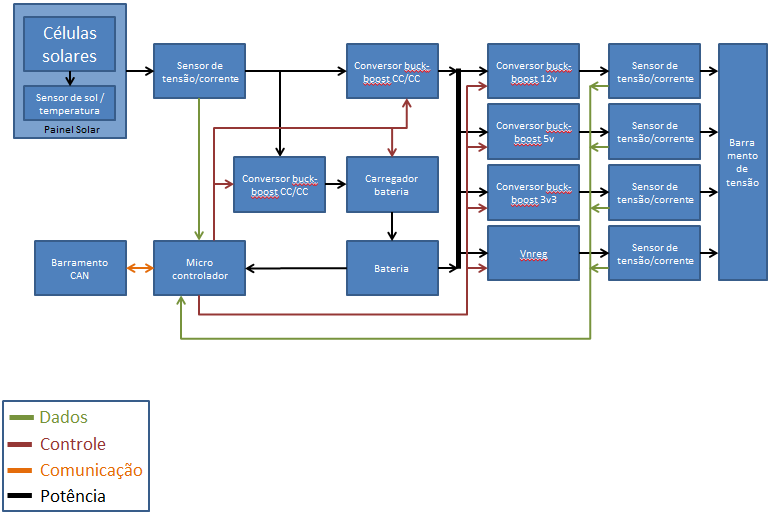
\includegraphics[width=1.0\linewidth]{./figs/diag_blocos_inicial}
			
		\begin{small}
			FONTE: Elaborado pelos autores.
		\end{small}		
	\end{figure}	
	\pagebreak

	Inicialmente, foi previsto a utilização de 4 placas com fotocélulas, as quais iriam gerar uma tensão no carregador de baterias e no barramento interno. A partir desse barramento a energia chegaria aos conversores sendo convertidas para 3,3V, 5V, 12V e uma tensão não regulada (V\textsubscript{nreg}). Essas tensões provenientes dos conversores, passariam pelos sensores de tensão e corrente chegando ao barramento externo, alimentando todos os subsistemas do \textit{CubeSat}.
	
	Nessa topologia quando o \textit{CubeSat} estivesse em região de sombra solar, ou seja, quando não tivesse incidência direta de luz nas suas fotocélulas, o microcontrolador faria o chaveamento para a bateria de 4,2V, dessa forma a bateria assumiria a responsabilidade de gerar a energia necessária para o funcionamento do sistema até que o \textit{CubeSat} voltasse a receber incidência de luz solar.
	
	Alguns fatores foram determinantes para a alteração da topologia utilizada no projeto.
	
	\begin{minipage}{7cm}	
		\begin{itemize}
			\item	Condições do espaço;
			\item	Falta de redundância;
			\item	Eficiência dos conversores;
		\end{itemize}
	\end{minipage}
	\begin{minipage}{7cm}
		\begin{itemize}
			\item	Adição do conversor \textit{backup};
			\item	Troca da bateria de 4,2V para 7,4V.
		\end{itemize}
	\end{minipage}
	\pagebreak
	
	Já na versão final do diagrama, representado na Figura \ref{Fig_Diag_Blocos_Final}, o projeto foi subdividido em três partes, sendo elas, a placa de controle, placa do carregador e as quatro placas de fotocélulas (+X, -X, +Y e -Y). Nas seções seguintes serão exibidos os estudos que justificaram as alterações realizadas.
 
\section[Definição dos componentes]{Definição dos componentes}\label{Sec_Def_Comp}

	A seguir será explicado de uma forma mais detalhada, como foram realizadas as escolhas dos principais componentes do projeto. Importante ressaltar que os projetos de \textit{CubeSats} possuem como premissa o conceito de ser um projeto de baixo custo, porém o referencial do custo utilizado são os custos de projetos de grandes satélites.
	
	Para a utilização dos componentes que suportem as condições impostas  no meio espacial, alguns fabricantes possuem linhas de produtos voltadas para utilização de componentes aeroespaciais que possuem um custo mais elevado em comparação aos componentes utilizados no mercado comum.

\subsection[Bateria]{Bateria} \label{Sec_Bateria}

	Como mencionado na Seção \ref{Sec_Bateria}, na Tabela \ref{Tab_Bateria}, foi escolhida a bateria do tipo íon-lítio. Essa definição foi baseada pela análise dos prós e contras desse modelo.
	
	\begin{minipage}{6cm}
		\begin{center}
			\textbf{PRÓS}
		\end{center}
		
		\begin{itemize}
			\item Alto ciclo de vida;
			\item Alta densidade energética;
			\item baixa auto-descarga mensal;
			\item Não apresenta necessidade de manutenção.
		\end{itemize}
	
	\end{minipage}
	\begin{minipage}{7cm}
		\begin{center}
			\textbf{CONTRAS}
		\end{center}
		
		\begin{itemize}
			\item Baixa tolerância para sobrecargas;
			\item Tempo para carga rápida;
			\item Preço elevado em comparação aos demais tipos.
		\end{itemize}
		
	\end{minipage}
		
	Foram utilizadas duas baterias de duas células que possuem 7,4V e 2000 mAh, sendo uma para o conjunto principal e a outra para o conjunto de redundância do Sistema de Gerenciamento de Energia para \textit{CubeSat}. Na Figura \ref{Fig_Bat_Sel}, é possível visualizar a bateria selecionada.
	
	\begin{figure}[th]
		\caption{BATERIA DE ÍON-LÍTIO SELECIONADA}
		\label{Fig_Bat_Sel}
		\centering
		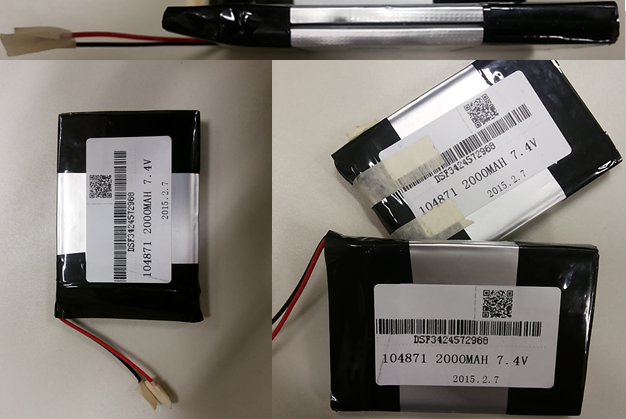
\includegraphics[width=0.8\linewidth]{./figs/cubesat_04}
			
		\begin{small}
			FONTE: Fotos tiradas pelos autores.
		\end{small}
	\end{figure}
	\pagebreak
		
\subsection[Fotocélulas]{Fotocélulas}\label{Sec_Cell}

	Após analisar os modelos dos principais fornecedores (Tabelas \ref{Tab_Spectro_Comp}, \ref{Tab_Emcore_Comp} e \ref{Tab_Azur_Comp}, Seção \ref{Cap_Cell}), foram solicitados orçamentos das fotocélulas para realizar o comparativo de preços e, por fim, realizar os procedimentos necessários para a aquisição das mesmas.
	
	O contato com a \textit{SpectroLab} não teve obteve sucesso, uma vez que a empresa não respondeu nenhuma das tentativas de contato realizadas. Já a solicitação do orçamento da \textit{SolAero Technologies} (antiga \textit{Emcore}) não caminhou conforme esperado, uma vez que entre as políticas de vendas da empresa existe a da prática de um pedido mínimo de \$7.500,00.
	
	A \textit{AzurSpace} enviou um orçamento dos modelos solicitados, conforme Tabela \ref{Tab_Orc_Cell}.
	
	\begin{table}[th]
	\caption{ORÇAMENTO DAS FOTOCÉLULAS DA \textit{AZURSPACE}}
	\label{Tab_Orc_Cell}
	\centering
	\begin{tabular}{p{3.0cm}|p{3.0cm}|p{3.0cm}|p{3.0cm}}
		\textbf{Modelo} & \textbf{Valor unitário} & \textbf{Frete} & \textit{\textbf{Lead time}}\\
		\hline
		3G28C & \euro 193,00 & \euro 195,00 & 8 a 10 semanas\\
		3G30C & \euro 198,00 & \euro 195,00 & 8 a 10 semanas\\

	\end{tabular}
	
	\begin{small}
	\vspace{3pt}
		FONTE: Elaborada pelos autores através do orçamento recebido pela \textit{AzurSpace}.
	\end{small}
	\end{table}	
	
	Devido ao alto custo e o grande \textit{lead time} da \textit{AzurSpace}, novas pesquisas foram feitas na tentativa de encontrar um novo fornecedor de fotocélulas com um custo mais acessível. Após uma busca detalhada em diversos grupos de discussões sobre o desenvolvimento de \textit{CubeSats}, foi encontrada no \textit{LinkedIn} a empresa \textbf{\textit{TrisolX}}.
	
	A \textit{TrisolX} é uma pequena empresa, localizada em Nova Iorque, que oferece uma alternativa acessível para projetos com orçamentos reduzidos. A empresa, vende a \textit{TrisolX Solar Wings}, que são fotocélulas cortadas a partir do modelo \textit{3G28C} da \textit{AzurSpace}.
	
	É o mesmo produto da \textit{AzurSpace}, porém com tamanho e formato diferentes, conforme Figura \ref{Fig_Cell_TrisolX}.
	
	\begin{figure}[th]
		\caption{MODELO DE FOTOCÉLULA DA \textit{TRISOLX}}
		\label{Fig_Cell_TrisolX}
		\centering
		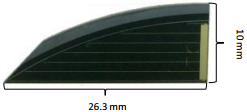
\includegraphics[width=0.5\linewidth]{./figs/TrisolX}
			
		\begin{small}
			FONTE: \textit{TrisolX}\textsuperscript{\cite{TrisolX}}
		\end{small}		
	\end{figure}	

	Foi solicitado um orçamento à \textit{TrisolX}, que prontamente foi recebido conforme Tabela \ref{Tab_Orc_TrisolX}.
	
	\begin{table}[th]
	\caption{ORÇAMENTO DAS FOTOCÉLULAS DA \textit{TRISOLX}}
	\label{Tab_Orc_TrisolX}
	\centering
	\begin{tabular}{p{3.5cm}|p{2.5cm}|p{1.5cm}|p{1.5cm}|p{2.0cm}}
		\textbf{Pacote} & \textbf{Quantidade} & \textbf{Valor} & \textbf{Frete} & \textbf{Prazo de entrega}\\
		\hline
		\textit{Sample Pack} & 5 células & \$25,00 &  \$68,00 & 2 semanas\\
		\textit{Starter Pack} & 25 células & \$100,00 &  \$68,00 & 2 semanas\\
		\textit{Development Pack} & 100 células & \$400,00 & \$68,00 & 2 semanas\\
	\end{tabular}
	
	\begin{small}
	\vspace{3pt}
		FONTE: Elaborada pelos autores através do orçamento recebedido pela \textit{TrisolX}.
	\end{small}
	
	\begin{footnotesize}
		NOTA: O modelo das fotocélulas comercializado pela \textit{TrisolX} é o \textit{3G28C} da \textit{AzurSpace}.
	\end{footnotesize}
	\end{table}	
	
	Tendo como objetivo inicial fazer a validação do sistema como um todo, realizar testes de pressão, temperatura e radiação, para fazer um levantamento completo do funcionamento do sistema, foi solicitado para a \textit{TrisolX} o \textit{Starter Pack}, conforme Tabela \ref{Tab_Orc_TrisolX}. Dessa forma foi possível ganhar experiência no manuseio das fotocélulas e validar o sistema, para depois fazer a aquisição das fotocélulas mais robustas da \textit{AzurSpace}.
	
\subsection[Componentes passivos]{Componentes passivos}
	
	Os componentes passivos foram selecionados de acordo com as Tabelas \ref{Tab_Resistores}, \ref{Tab_Indutores} e \ref{Tab_Capacitores}. Essa seleção tomou o cuidado de selecionar componentes que tivessem as características citadas na Seção \ref{Cap_Passivo}, ou seja, possuem um grande \textit{range} de temperatura de operação, uma certa tolerância a radiação, além do dimensional \textit{SMD}. Os capacitores possuem baixo \textit{ESR}, coeficiente de temperatura X7R, além de serem componentes do tipo \textit{SMD}.
	
	\begin{table}[th]
	\caption{RESISTORES}
	\label{Tab_Resistores}
	\centering
		\begin{tabular}{p{1.5cm}|p{2cm}|p{1.2cm}}
			\textbf{Valor} & \textbf{\textit{Package}} & \textbf{Qtdd.}\\
			\hline
			0,1 $ \Omega $ & \textit{SMD} 2818 & 12 un.\\
			470 $ \Omega $ & \textit{SMD} 0805 & 24 un.\\
			100 $ \Omega $ & \textit{SMD} 0805 & 4 un.\\
			100 k$ \Omega $ & \textit{SMD} 0805 & 4 un.\\
			10 k$ \Omega $ & \textit{SMD} 0805 & 16 un.\\
			10,7 k$ \Omega $ & \textit{SMD} 0805 & 4 un.\\
			115 k$ \Omega $ & \textit{SMD} 0805 & 12 un.\\
			120 $ \Omega $ & \textit{SMD} 0805 & 4 un.\\
			13,3 k$ \Omega $ & \textit{SMD} 0805 & 4 un.\\
			17,4 k$ \Omega $ & \textit{SMD} 0805 & 24 un.\\
			1 k$ \Omega $ & \textit{SMD} 0805 & 25 un.\\
			1,5 k$ \Omega $ & \textit{SMD} 0805 & 16 un.\\
			0,033 $ \Omega $ & \textit{SMD} 2818 & 4 un.\\
			220 k$ \Omega $ & \textit{SMD} 0805 & 4 un.\\
			22 k$ \Omega $ & \textit{SMD} 0805 & 20 un.\\
			2,49 k$ \Omega $ & \textit{SMD} 0805 & 64 un.\\
			2,2 k$ \Omega $ & \textit{SMD} 0805 & 4 un.\\
			3,4 k$ \Omega $ & \textit{SMD} 0805 & 4 un.\\
			33,2 k$ \Omega $ & \textit{SMD} 0805 & 4 un.\\
			56,2 k$ \Omega $ & \textit{SMD} 0805 & 8 un.\\
			680 k$ \Omega $ & \textit{SMD} 0805 & 4 un.\\
			71,5 k$ \Omega $ & \textit{SMD} 0805 & 8 un.\\
			8,45 k$ \Omega $ & \textit{SMD} 0805 & 32 un.\\
		\end{tabular}	
	
	\begin{small}
	\vspace{3pt}
		FONTE: Elaborada pelos autores.
	\end{small}
	\end{table}
	\pagebreak
	
	\begin{table}[th]
	\caption{INDUTORES}
	\label{Tab_Indutores}
	\centering
		\begin{tabular}{p{1.5cm}|p{5.5cm}|p{1.2cm}}
			\textbf{Valor} & \textbf{\textit{Package}} & \textbf{Qtdd.}\\
			\hline
			10 $ \mu $H & 6.86mm x 6.47mm x 3mm & 4 un.\\
			2,2 $ \mu $H & 5.49mm x 5.18mm x 2mm & 4 un.\\
			3,3 $ \mu $H & 6.86mm x 6.47mm x 3mm & 4 un.\\
			33 $ \mu $H & 10.8mm x 10.8mm x 4.16mm & 16 un.\\
		\end{tabular}	
	
	\begin{small}
	\vspace{3pt}
		FONTE: Elaborada pelos autores.
	\end{small}
	\end{table}	
	
	\begin{table}[th]
	\caption{CAPACITORES}
	\label{Tab_Capacitores}
	\centering
		\begin{tabular}{p{2cm}|p{2cm}|p{1.3cm}}
			\textbf{Valor} & \textbf{\textit{Package}} & \textbf{Qtdd.}\\
			\hline
			3300 pF & \textit{SMD} 0805 & 148 un.\\
			0,022 $\mu$F & \textit{SMD} 0805 & 4 un.\\
			1000 pF & \textit{SMD} 0805 & 16 un.\\
			100 nF & \textit{SMD} 0805 & 12 un.\\
			10 nF & \textit{SMD} 0805 & 4 un.\\
			10 $\mu$F & \textit{Case R} & 4 un.\\
			1500 pF & \textit{SMD} 0805 & 4 un.\\
			1 $\mu$F & \textit{SMD} 0805 & 32 un.\\
			2,2 nF & \textit{SMD} 0805 & 4 un.\\
			220 nF & \textit{SMD} 0805 & 28 un.\\
			22 $\mu$F & \textit{Case C} & 4 un.\\
			47 nF & \textit{SMD} 0805 & 16 un.\\
			47 $\mu$F & \textit{Case C} & 4 un.\\
		\end{tabular}	
	
	\begin{small}
	\vspace{3pt}
		FONTE: Elaborada pelos autores.
	\end{small}
	\end{table}
	\pagebreak

\subsection[Semicondutores]{Semicondutores}\label{Sec_Semicondutores}

	Inicialmente foram procurados diversos circuitos integrados de conversores capazes de realizar a elevação e diminuição da tensão de saída para a topologia inicial, onde existiria duas baterias em série com 4,2V. Porém após diversas horas de estudos não foram encontrados conversores \textit{Boost} capazes de realizar grandes elevações com alta eficiência. Somente os conversores com uma tensão de entrada superior aos 4,2V poderiam atender a especificação do projeto com a grande eficiência desejada.
	
	Dessa forma, foi alterada a topologia do projeto, onde as baterias de 4,2V, foram substituídas pela bateria de duas células em série de 7,4V, definida na Seção \ref{Sec_Bateria}.
	
	Durante as pesquisas, foi encontrado o projeto \textit{Open Source Satellite Initiative}. Na \textit{wikipage} deste projeto estava disponibilizado um \textit{link} para uma base de dados que contém informações de diversos testes de radiação realizados na \textit{NASA Goddard Space Flight Center}.\textsuperscript{\cite{OSSI}}\textsuperscript{\cite{OSSI2}}\textsuperscript{\cite{OSSI3}}
	
	Nessa base de dados foram encontrados alguns conversores que poderiam ser utilizados no desenvolvimento do projeto, como por exemplo o \textit{Buck} TPS50601-SP da \textit{Texas Instruments}. Porém devido ao alto custo dos componentes presentes nessa lista o componente não foi uma solução viável ao projeto.
	
	Reiniciada a etapa de pesquisas, foi encontrado o \textit{WEBENCH Design Center}, software \textit{online} da \textit{Texas Instruments}, no qual é possível inserir os parâmetros que se deseja de um conversor, como por exemplo, tensão de entrada e tensão de saída, e o software consulta sua base de dados para encontrar o conversor especificado e ainda reproduz o circuito de \textit{datasheet} da aplicação. Através do auxilio do \textit{WEBENCH Design Center}, foram identificados os seguintes conversores LM3488 (\textit{boost}) e o TPS563200 (\textit{buck}).
	
	Para a definição do conversor \textit{backup}, foi pesquisado um único conversor com diversas saídas, dessa forma apenas um circuito integrado seria capaz de devolver as tensões de 3,3V, 5V e 12V. A princípio foram encontrados algumas opções desses conversores com múltiplas saídas, porém todos os encontrados eram de 4 saídas. Após uma busca mais criteriosa, foi encontrado na \textit{Linear Technology} o LT1941 que possui as três saídas desejadas, sendo uma saída \textit{Boost} e duas saídas \textit{Buck}. Com a ajuda do \textit{LTspice IV}, software da própria \textit{Linear}, foi possível trabalhar em cima do \textit{application note} do \textit{datasheet} do componente para poder adaptá-lo as necessidades do projeto do Sistema de Gerenciamento de Energia para \textit{CubeSats}.

	Para a definição do carregador de baterias foram tomadas todas as precauções para se obter um carregador com o recurso de monitoramento da carga e com uma boa eficiência, dessa forma foi selecionado o BQ24005 da \textit{Texas Instruments}, dentre suas características destacam-se:
	
	\begin{itemize}
		\item Baixo consumo em \textit{sleep mode};
		\item Regulação de tensão de alta precisão ($\pm$ 1\%);
		\item Carregamento seguro com temporizador durante o pré-condicionamento;
		\item Dissipação de calor durante a fase inicial da carga;
		\item Entre outras.
	\end{itemize}
	
\subsection[Lista de componentes]{Lista de componentes}

	Após a compilação de todos os componentes foi finalizada a lista de componentes necessários para o seguimento do projeto, também foi levada em consideração a questão financeira, portanto, alguns componentes apresentados nesta lista podem ser substituídos após a realização de todos os ensaios e validações.
		
	Foi solicitado um orçamento para a \textit{Farnell}, que devido a sua grande estrutura e interligação entre os estoques nacionais e internacionais, tinha a disposição praticamente todos os componentes necessários com exceção do carregador de bateria (BQ24005). O orçamento ficou R\$ 2.065,66, conforme pode ser visto no Apêndice \ref{Orçamento}.	
	
	Nesse capítulo foi ilustrado o processo de seleção dos componentes necessários para a construção do Sistema de Gerenciamento de Energia para \textit{CubeSat}. No capítulo seguinte serão abordados os tópicos de desenvolvimento de \textit{hardware} e \textit{software} utilizado no decorrer do projeto.
	
\section[Desenvolvimento de hardware]{Desenvolvimento de \textit{hardware}}

	O desenvolvimento de hardware se resume ao processo de elaboração de circuito eletrônico, \textit{layout} de \textit{PCB}, montagem e testes das placas eletrônicas. Nesta etapa será mostrado como foram realizadas as fases de montagem das placas, a depuração e testes de funcionalidades para a prova de conceito desenvolvida. Pela complexidade do sistema proposto, o mesmo será explicado de forma separada entre as placas desenvolvidas, sendo elas:
	
	\begin{enumerate}
		\item Painel Solar;
		\item Placa do Carregador;
		\item Placa de Controle.
	\end{enumerate}

	Para o desenvolvimento dos circuitos e dos \textit{layouts} das \textit{PCB}, as ferramentas utilizadas foram o \textit{CadSoft EAGLE PCB Design Software} na versão \textit{Light Edition Free} e \textit{SketchUp} também na versão gratuita para a visualização dos modelos 3D.
	
\subsection[Painel Solar]{Painel Solar}

	Conforme definido na Seção \ref{Sec_Cell}, foram utilizadas as fotocélulas da \textit{TrisolX}. Para realizar o carregamento da bateria é necessário que a tensão gerada pelo painel solar seja de 8,4V a 10V. 
	
	Como cada fotocélula consegue fornecer até 2,33V, foi realizado um arranjo com quatro células em série, conseguindo fornecer uma tensão de 9,32V. Foram implementados, em paralelo, seis conjuntos com quatro fotocélulas em série, totalizando 24 fotocélulas no painel solar. Foram utilizados diodos de \textit{bypass} para evitar danos e perdas de potência do sistema devido a diferenças de características elétricas das fotocélulas, conforme Figura \ref{Fig_Circ_Cell}.
	
	\begin{figure}[th]
		\caption{CIRCUITO ELÉTRICO PAINEL SOLAR}
		\label{Fig_Circ_Cell}
		\centering
		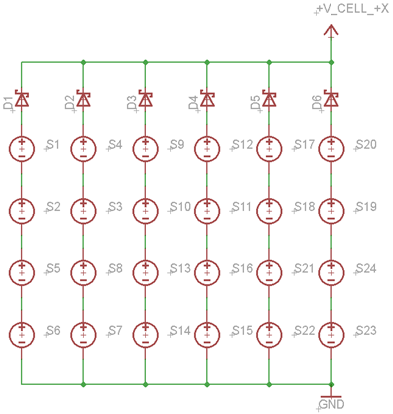
\includegraphics[width=0.6\linewidth]{./figs/circ_cell}
			
		\begin{small}
			FONTE: Elaborado pelos autores.
		\end{small}
	\end{figure}
	\pagebreak
	
	Considerando a área total disponível para uma face do painel solar, o \textit{layout} foi elaborado de forma que o arranjo das 24 fotocélulas ficassem melhor alocadas na placa, conforme Figura \ref{Fig_layout_cell}.
	
	\begin{figure}[th]
		\caption{\textit{LAYOUT} DO PAINEL SOLAR}
		\label{Fig_layout_cell}
		\centering
		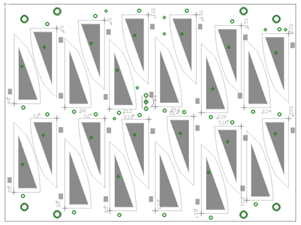
\includegraphics[width=0.6\linewidth]{./figs/layout_cell}
			
		\begin{small}
			FONTE: Elaborado pelos autores.
		\end{small}
	\end{figure}
	
	Para realizar a montagem do painel solar foi necessário muito cuidado pois as fotocélulas são extremamente frágeis e quebram com facilidade. Outro fator importante é a utilização de luvas, dessa forma evita-se que durante o manuseio das fotocélulas, as mesmas fiquem engorduradas, o que implica em queda de rendimento. Visando contornar os problemas apresentados, optou-se por realizar a soldagem em um forne de refusão modelo \textit{ProtoFlow E}, disponível no laboratório da Escola de Engenharia Mauá. Porém antes da placa ir para o forno de refusão, foi necessário estanhar os \textit{pads} das fotocélulas.\footnote{No Apêndice \ref{ProtoFlow} é possível visualizar o forno de refusão \textit{ProtoFlow E}, a configuração utilizada e algumas etapas do processo.}

	\begin{figure}[th]
		\caption{PAINEL SOLAR FINALIZADO}
		\centering
		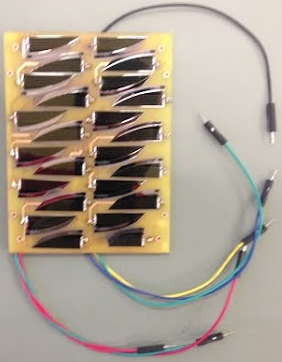
\includegraphics[width=0.75\linewidth]{./figs/painel_solar}
		
		\begin{small}
			FONTE: Foto tirada pelos autores.
		\end{small}	
	\end{figure}
	
	Para validar a montagem do painel solar foi montado o \textit{setup} representado na Figura \ref{Fig_setup_cell}.
	
	\begin{figure}[th]
		\caption{ESQUEMA DO \textit{SETUP} DE VALIDAÇÃO DO PAINEL SOLAR}
		\centering
		\label{Fig_setup_cell}
		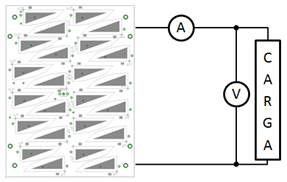
\includegraphics[width=0.8\linewidth]{./figs/setup_solar}
		
		\begin{small}
			FONTE: Elaborado pelos autores.
		\end{small}	
	\end{figure}
	\pagebreak
	
	O procedimento utilizado para o teste do painel solar consistiu em variar a resistência de carga enquanto a tensão e corrente geradas eram monitoradas.
	 
	Medições preliminares foram realizadas com lâmpadas incandescentes de 100W, colocadas a 25cm de distância do painel, as fotocélulas ficaram expostas a luz e ao calor. Porém como o espectro de uma lâmpada incandescente não é o mesmo da luz solar, somado ao efeito do coeficiente de temperatura de -6,1mV/ºC das fotocélulas e a exposição de calor, resultaram em medidas não representativas.
	
	Novas medições foram realizadas utilizando luz solar em um dia de céu limpo com temperatura ambiente de 27ºC. 
Este procedimento foi feito para duas condições distintas, a primeira considerando apenas a geração de energia de uma única fotocélula, e a segunda considerando a energia gerada por 4 células em série.

	\begin{itemize}
		\item Ensaio com uma fotocélula.
	\end{itemize}
	
	Realizado o cálculo para encontrar a resistência de carga na condição de máxima transferência de potencia.
	
	Dados do fabricante:
	\begin{itemize}
		\item \textit{Voltage (Max Power)} = 2,33V;
		\item \textit{Current (Max Power)} = 14,6mA.
	\end{itemize}
	
	\begin{eqnarray}
		R_{carga} = \dfrac{V_{Max Power}}{I_{Max Power}}		
	\end{eqnarray}
	
	\begin{eqnarray*}
		R_{carga} = \dfrac{2,33}{14,6\times10^{-3}} \Rightarrow R_{carga} = 159,58\Omega		
	\end{eqnarray*}
	
	O cálculo para obter a máxima transferência de potencia é:
	
	\begin{eqnarray}
		P_{Max} = V_{Max Power} \cdot I_{Max Power}	
	\end{eqnarray}
	
	\begin{eqnarray*}
		P_{Max} = 2,33 \cdot 14,6\times10^{-3} \Rightarrow P_{Max} = 34,01mW
	\end{eqnarray*}
	
\subsection[Placa do carregador]{Placa do carregador}

	A placa do carregador é onde está alocado o conversor \textit{backup}, que fornece energia ao barramento de saída caso ocorra alguma falha no sistema principal, além de contar com um multiplexador analógico que realiza as leituras dos sensores de temperatura dos painéis solares conforme o microcontrolador seleciona o painel desejado.
	
	A Figura \ref{Fig_circ_conv} mostra o circuito do LT1941 da \textit{Linear Technology} utilizado para o conversor \textit{backup} , conforme definido na Seção \ref{Sec_Semicondutores}.
	
	\begin{figure}[th]
		\caption{CIRCUITO ELÉTRICO DO CONVERSOR \textit{BACKUP}}
		\label{Fig_circ_conv}
		\centering
		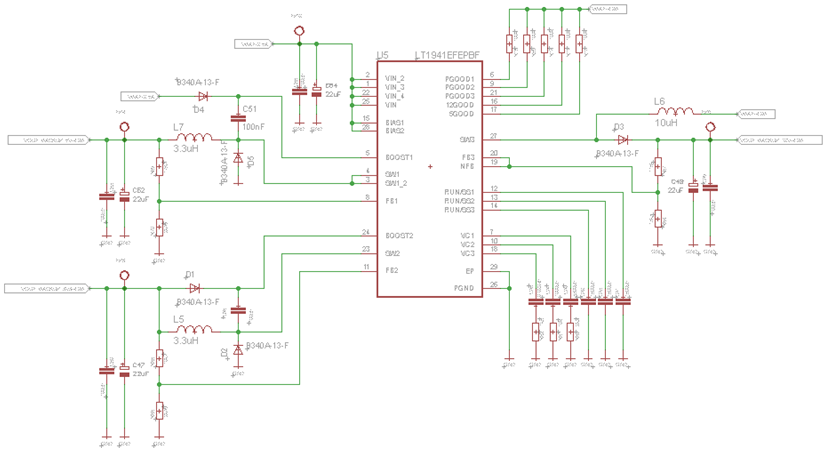
\includegraphics[width=0.9\linewidth]{./figs/circ_back}
			
		\begin{small}
			FONTE: Elaborado pelos autores.
		\end{small}
	\end{figure}
	
	Este conversor foi utilizado pois a frequência de chaveamento de 1,1MHz possibilitou o uso de pequenos indutores e capacitores, tornando eficaz seu uso no Sistema de Gerenciamento de Energia para \textit{CubeSats}. Os demais componentes utilizados foram utilizados de acordo com os dados do fabricante.
	
	O resultado do \textit{layout} da placa pode ser visto na Figura \ref{Fig_layout_carg}, onde buscou-se obter um bom aproveitamento da área disponível da \textit{PCB} de forma a facilitar a montagem da placa na estrutura do \textit{CubeSat}.
	
	\begin{figure}[th]
		\caption{\textit{LAYOUT} DETALHADO DA PLACA DO CARREGADOR}
		\label{Fig_layout_carg}
		\centering
		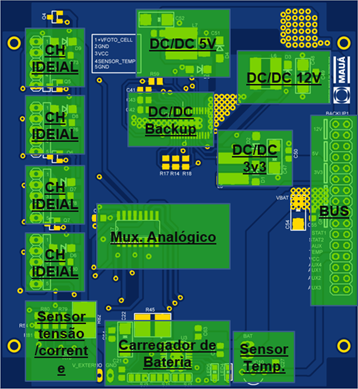
\includegraphics[width=0.37\linewidth]{./figs/layout_carg}
			
		\begin{small}
			FONTE: Elaborado pelos autores.
		\end{small}
	\end{figure}
	
	A Figura \ref{Fig_layout_carg} foi editada de forma a facilitar a localização de cada conjunto utilizado na placa.\footnote{No Apêndice \ref{P_Carreg} é possível visualizar o \textit{layout} sem os blocos de identificação dos componentes.}
	
	Para a montagem da placa do carregador foi necessário apenas utilizar uma estação de solda para realizar o processo de soldagem de todos os componentes \textit{SMD}.
	
	\begin{figure}[th]
		\caption{PLACA DO CARREGADOR FINALIZADA}
		\label{Fig_placa_carg}
		\centering
		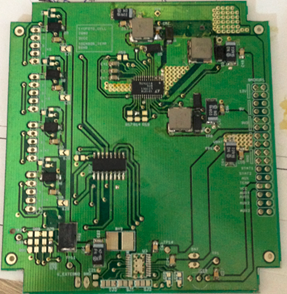
\includegraphics[width=0.37\linewidth]{./figs/placa_carreg}
			
		\begin{small}
			FONTE: Foto tirada pelos autores.
		\end{small}
	\end{figure}
	\pagebreak
	
\subsection[Placa de controle]{Placa de controle}

	A placa de controle é responsável pelos conversores principal, chave inteligente de baixas perdas (chaves ideais) e sensores de tensão e corrente, além do microcontrolador que realiza todo o monitoramento do sistema.
	
	Para o funcionamento da chave ideal, é necessário um circuito, apresentado na Figura \ref{Fig_chave}, que realize a isolação entre a fonte principal e a fonte \textit{backup} com baixa perda de tensão. Esse circuito utiliza o circuito integrado LTC4412, definido na Seção \ref{Sec_Semicondutores}, que comparado a um diodo convencional possui uma queda de tensão muito inferior, sendo de aproximadamente 20mV.
	
	\begin{figure}[th]
		\caption{CIRCUITO ELÉTRICO DA CHAVE IDEAL}
		\label{Fig_chave}
		\centering
		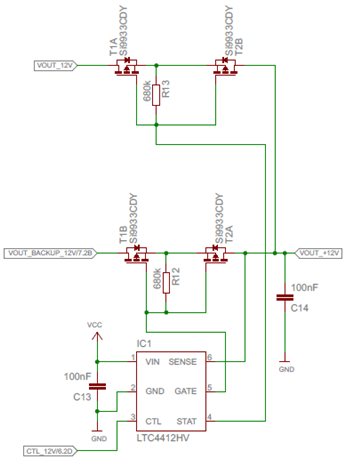
\includegraphics[width=0.5\linewidth]{./figs/chave_id}
			
		\begin{small}
			FONTE: Elaborado pelos autores.
		\end{small}
	\end{figure}

	Para o desenvolvimento do \textit{layout} da placa de controle, Figura \ref{Fig_pl_cont}, buscou-se obter o máximo aproveitamento da área disponível da \textit{PCB}, de forma análoga a placa do carregador, a facilidade de montagem da placa na estrutura foi levada em consideração.
	
	\begin{figure}[th]
		\caption{\textit{LAYOUT} DA PLACA DE CONTROLE}
		\label{Fig_pl_cont}
		\centering
		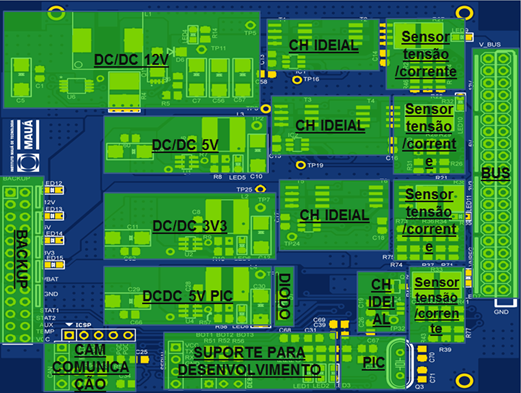
\includegraphics[width=0.6\linewidth]{./figs/pl_cont}
			
		\begin{small}
			FONTE: Elaborado pelos autores.
		\end{small}
	\end{figure}
	\pagebreak
	A Figura \ref{Fig_pl_cont} foi editada de forma a facilitar a localização de cada conjunto utilizado na placa.\footnote{No Apêndice \ref{P_Cont} é possível visualizar o \textit{layout} sem os blocos de identificação dos componentes.}
	
	Para a montagem da placa de controle foi necessário apenas utilizar uma estação de solda para realizar o processo de soldagem de todos os componentes \textit{SMD}.
	
	\begin{figure}[th]
		\caption{PLACA DE CONTROLE FINALIZADA - VISTA SUPERIOR}
		\label{Fig_esq_cont}
		\centering
		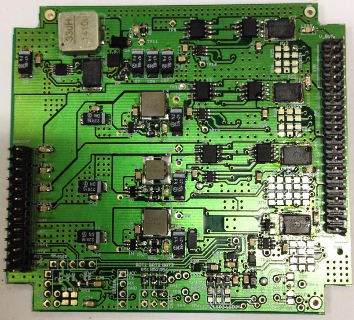
\includegraphics[width=0.6\linewidth]{./figs/cont_top}
			
		\begin{small}
			FONTE: Foto tirada pelos autores.
		\end{small}
	\end{figure}
	
	\begin{figure}[th]
		\caption{PLACA DE CONTROLE FINALIZADA - VISTA INFERIOR}
		\label{Fig_esq_cont}
		\centering
		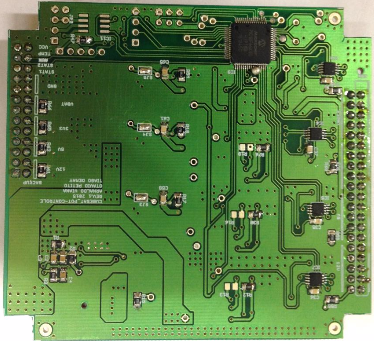
\includegraphics[width=0.6\linewidth]{./figs/cont_bottom}
			
		\begin{small}
			FONTE: Foto tirada pelos autores.
		\end{small}
	\end{figure}
	\pagebreak
	Para o ensaio dos conversores principais foi montado o esquema da Figura \ref{Fig_esq_cont}, para simular a bateria foi utilizada uma fonte de bancada, para a carga foi utilizado o uma década resistiva. O método para ensaio convencionado foi regular a tensão da fonte em uma tensão compatível com a da bateria de 7,4V e variar a resistência de carga de forma gradativa até obter a corrente nominal do conversor de tensão.
		
	\begin{figure}[th]
		\caption{ESQUEMA DE TESTES DA PLACA DE CONTROLE}
		\label{Fig_esq_cont}
		\centering
		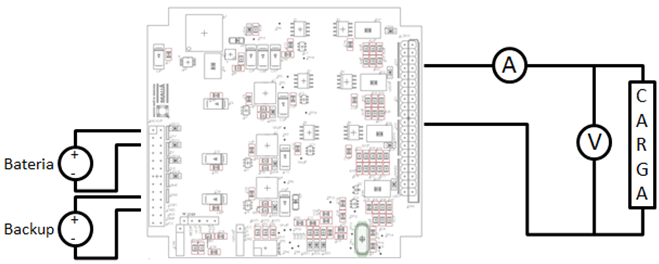
\includegraphics[width=1.0\linewidth]{./figs/esq_cont}
			
		\begin{small}
			FONTE: Elaborado pelos autores.
		\end{small}
	\end{figure}
	
	O ensaio foi realizado simulando três situações em que a bateria pode operar, variando uma fonte ajustável para as seguintes situações:

	\begin{itemize}
		\item 8,4V - bateria completamente carregada;
		\item 8,0V - bateria carregada;
		\item 7,4V - bateria descarregada.
	\end{itemize}
	
	Variando a resistência de carga, foram medidas corrente e tensão em 10 pontos distintos em toda a faixa de operação especificada, 12V/1A, 5V/2A, 3,3V/3A. Para o conversor de 5V foi utilizado as resistências de carga conforme Tabela \ref{Tab_res_teste}.
	
	\begin{table}[th]
	\caption{RESISTÊNCIAS DE CARGA UTILIZADAS NO TESTE}
	\label{Tab_res_teste}
	\centering
		\begin{tabular}{p{1.3cm}|p{1.3cm}}
			\textbf{R$_{carga}$} & \textbf{R$_{carga}$}\\
			\hline
			1k$\Omega$ & 7$\Omega$\\
			100$\Omega$ & 5$\Omega$\\
			50$\Omega$ & 4$\Omega$\\
			20$\Omega$ & 3$\Omega$\\
			10$\Omega$ & 2$\Omega$\\
		\end{tabular}	
	
	\begin{small}
	\vspace{3pt}
		FONTE: Elaborada pelos autores.
	\end{small}
	\end{table}
	
	Para realizar o ensaio, o \textit{setup} representado na Figura \ref{Fig_setup_cont} foi montado.
	
	\begin{figure}[th]
		\caption{\textit{SETUP} DE TESTES DA PLACA DE CONTROLE}
		\label{Fig_setup_cont}
		\centering
		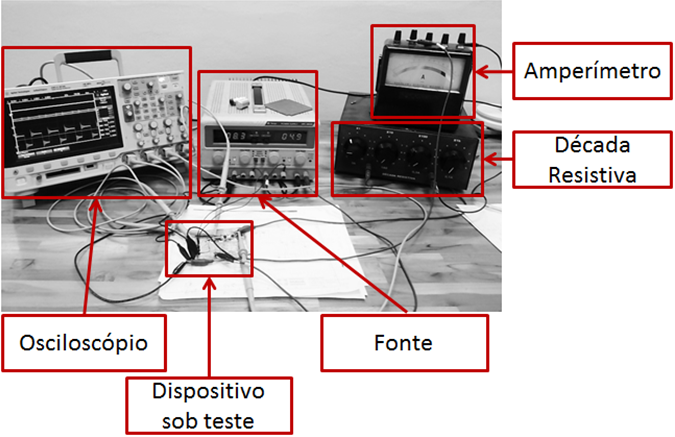
\includegraphics[width=1\linewidth]{./figs/setup_cont}
			
		\begin{small}
			FONTE: Elaborado pelos autores.
		\end{small}
	\end{figure}
	\pagebreak
	
	Com o osciloscópio foram monitorados os pontos identificados na Figura \ref{Fig_circ_test_cont}.\footnote{No Apêndice \ref{T_Cont} é possível visualizar os pontos utilizados para teste no modelo 3D da placa de controle.}
	
	\begin{figure}[th]
		\caption{CIRCUITO DE TESTES DA PLACA DE CONTROLE}
		\label{Fig_circ_test_cont}
		\centering
		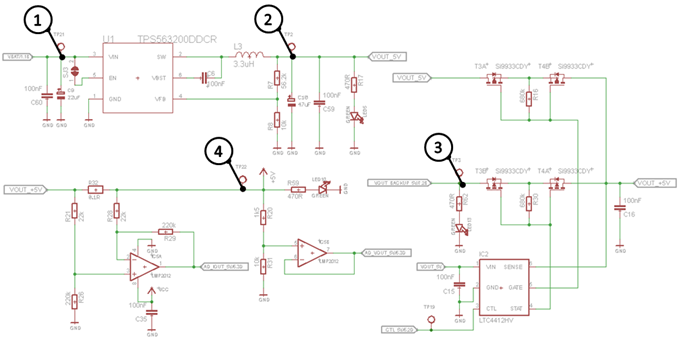
\includegraphics[width=1\linewidth]{./figs/circ_test_cont}
			
		\begin{small}
			FONTE: Elaborado pelos autores.
		\end{small}
	\end{figure}
	
	\begin{enumerate}
		\item Tensão de entrada da fonte principal;
		\item Tensão de saída do conversor principal;
		\item Tensão \textit{backup} na entrada da chave;
		\item Tensão de saída no barramento.
	\end{enumerate}
	
\section[Desenvolvimento de software]{Desenvolvimento de \textit{software}}

	Para o funcionamento do \textit{CubeSat} foi desenvolvido um \textit{software} de gerenciamento do sistema com base em linguagem C, que foi escolhida em função de se tratar de uma das linguagens mais populares, existindo poucas arquiteturas para as quais não existam compiladores. 
	
	Como plataforma de desenvolvimento foi selecionado o \textit{MPlab-X} que é distribuída gratuitamente pela empresa \textit{Microchip Technology}, que integra diversos ambientes de trabalho para programação, simulação e gravação de microcontroladores. 
	
	Conforme definição na Seção \ref{Sec_Semicondutores}, o microcontrolador usado foi o PIC18F66K80 e o gravador utilizado foi o \textit{PICkit 3 In-Circuit Debugger} ambos da \textit{Microchip Technology}.
	
\subsection[Fluxograma geral do software]{Fluxograma geral do \textit{software}}

	Como método de programação foi utilizado linguagem estruturada, ou seja, por tratar-se de um programa que interage com mais de um periférico, o programa foi "desconstruído" em partes, facilitando a programação em blocos, elas tornaram-se partes inteligíveis e fáceis de serem manipuladas. Isso faz com que o programador saiba o que ocorre em cada bloco do sistema, assim caso seja necessária alguma modificação no código isso ocorrerá de forma fácil e ágil, podendo ser visualizado na Figura \ref{Fig_fluxo_simples}.
	
	\begin{figure}[th]
		\caption{FLUXOGRAMA GERAL DO \textit{SOFTWARE}}
		\label{Fig_fluxo_simples}
		\centering
		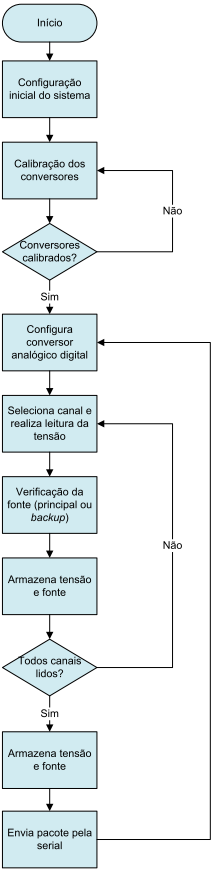
\includegraphics[width=0.28\linewidth]{./figs/fluxo_simples}
			
		\begin{small}
			FONTE: Elaborado pelos autores.
		\end{small}
	\end{figure}
	\pagebreak
	
	O programa inicia configurando o sistema para ser utilizado, com a utilização dos periféricos de transmissão serial e conversor analógico-digital para implementar as funções necessárias ao software, o sistema configura esses periféricos para uso. Logo em seguida calibra a leitura das tensões de todos os conversores utilizados.
	
	A telemetria funciona dentro de um laço de repetição simples, onde os canais dos conversores são alterados e lidos um a um, guardando a informação de tipo (entenda: valor lido que mostra se a fonte é principal ou \textit{backup}) e o valor das tensões lidas num vetor de dados, esse vetor é "bufferizado" e enviado via transmissão serial para a máquina conectada, que simula um computador de bordo (\textit{DPU}).  

\subsection[Fluxograma detalhado do software]{Fluxograma detalhado do \textit{software}}

	Antes de começar a programação dos conversores analógicos para digital (\textit{ADC}), identificando a necessidade que era preciso um meio de depurar o código para saber o que acontecia dentro do microcontrolador e como o \textit{firmware} estaria se comportando, além de facilitar a implementação do código, a comunicação serial é uma das melhores ferramentas de depuração quando se trata de sistemas embarcados.
	
	Para tal implementação foi utilizada a biblioteca do compilador \textit{XC8} para microcontroladores da família do PIC18. Outra boa prática utilizada foi o desenvolvimento estruturado do \textit{firmware}, ou seja, foi a utilização de arquivos dos tipos \textit{header (.h)} e \textit{sources (.s)}.
	
	\begin{figure}[th]
		\caption{FLUXOGRAMA DETALHADO DO \textit{SOFTWARE}}
		\label{Fig_fluxo_detalhado}
		\centering
		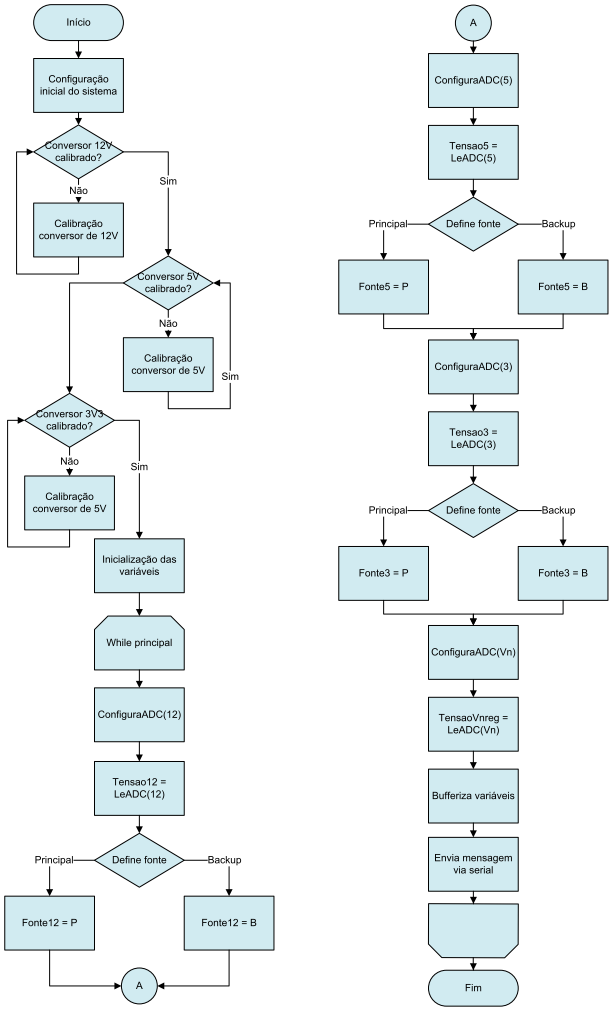
\includegraphics[width=0.75\linewidth]{./figs/fluxo_detalhado}
			
		\begin{small}
			FONTE: Elaborado pelos autores.
		\end{small}
	\end{figure}
	\pagebreak

	A configuração inicial, chamado de InitBoard no código, configura o \textit{clock} à 8MHz (oscilador interno do PIC), desliga os comparadores afim de minimizar possíveis incompatibilidades nos pinos do microcontrolador. Realiza a configuração dos registradores que definem os pinos como entradas e saídas, os chamados registradores \textit{TRIS}. Define também que a chave ideal ligue o barramento principal e por fim configura a transmissão serial que será utilizada como \textit{USART} (\textit{Universal Synchronous Asynchronous Receiver Transmitter}), configurado internamente na forma síncrona, uma ponta é mestre e a outra escravo. Um fio é utilizado para tráfego de dados, em regime \textit{half-duplex}, ou seja, nos dois sentidos, mas um sentido de cada vez. O outro fio é usado para pulsos de \textit{clock} emitidos pelo dispositivo mestre.
	
	A calibração dos conversores tem a função de guardar na memória do microcontrolador o valor correspondente de cada tensão, que irá para o barramento de saída, e o tipo principal ou \textit{backup}, para que o PIC possa identificar na transmissão serial qual a fonte que gera aquela tensão no barramento de saída.
	
	A calibração ocorre da seguinte maneira: o microcontrolador força a chave ideal a fornecer o valor da tensão da fonte principal que é armazenada, em seguida o microcontrolador passa a chave ideal para o fornecimento da tensão para o \textit{backup} e faz um comparativo para validar se o valor da tensão principal é superior ao valor da tensão do \textit{backup}. Realizando esse ciclo para as três tensões oferecidas no barramento.	
	
	A configuração do conversor analógico para digital, foi realizada utilizando-se uma lógica de mascaramento \textit{AND} utilizada para configurar os registradores do módulo \textit{ADC} (\textit{Analogic Digital Converter}) sem a necessidade de configurar \textit{bit} por \textit{bit}. A função \textit{OpenADC} utiliza as variáveis config1, 2 e 3 feitas neste processo de mascaramento e finaliza a configuração, deixando o \textit{ADC} pronto para ser utilizado no pino (\textit{Channel}) selecionado.
	
	A conversão tem seu início com a função \textit{ConvertADC} que espera o \textit{buffer} do \textit{ADC} ser liberado, assim que a conversão fica pronta o \textit{flag} do \textit{bit1} do registrador \textit{ADCON0} vai automaticamente para nível lógico baixo (zero digital), a função \textit{ReadADC}, faz a leitura e guarda seu valor na variável de resultado do conversor selecionado, este procedimento é executado 16 vezes e é tirado uma média dos valores, para uma maior precisão dos dados colhidos.
	
	Os dados são "bufferizados" de acordo com o protocolo \textit{topx}, este protocolo cria um vetor com as informações de tensões e tipos (principal ou \textit{backup}), e os transmite para a estação de trabalho conectada a porta serial, que pode utilizar os dados da maneira que desejar. 

\subsection[Protocolo de comunicação serial]{Protocolo de comunicação serial}

	O protocolo \textit{topx} foi desenvolvido para realizar o envio das mensagens enviadas pela serial. É um protocolo composto por 25 \textit{bytes}.\footnote{No Apêndice \ref{Prot_Serial} é possível visualizar a estrutura \textit{byte-to-byte} do protocolo.}
	
	A estrutura do protocolo respeita a Tabela \ref{Tab_prot}.
	
	\begin{table}[th]
	\caption{ESTRUTURA DO PROTOCOLO \textit{TOPX}}
	\label{Tab_prot}
	\centering
		\begin{tabular}{|c|c|}
			\hline
			Indicador tensão 12V & 1 \textit{byte} \\
			\hline
			Indicador fonte 12V & 1 \textit{byte} \\
			\hline
			Valor tensão 12V & 4 \textit{bytes} \\
			\hline
			Indicador tensão 5V & 1 \textit{byte} \\
			\hline
			Indicador fonte 5V & 1 \textit{byte} \\
			\hline
			Valor tensão 5V & 4 \textit{bytes} \\
			\hline
			Indicador tensão 3,3V & 1 \textit{byte} \\
			\hline
			Indicador fonte 3,3V & 1 \textit{byte} \\
			\hline
			Valor tensão 3,3V & 4 \textit{bytes} \\
			\hline
			Indicador tensão V$ _{nreg} $ & 1 \textit{byte} \\
			\hline
			Indicador fonte V$ _{nreg} $ & 1 \textit{byte} \\
			\hline
			Valor tensão V$ _{nreg} $ & 4 \textit{bytes} \\
			\hline
			Terminador de mensagem & 1 \textit{byte} \\
			\hline
		\end{tabular}	
	
	\begin{small}
	\vspace{3pt}
		FONTE: Elaborada pelos autores.
	\end{small}
	\end{table}

\section[Simulador de falhas e Simulink]{Simulador de falhas e \textit{Simulink}}

	Com o intuito de validar a solução proposta, foi desenvolvido um simulador de falhas e criado no ambiente do \textit{Simulink} uma interface onde é possível visualizar o funcionamento do Sistema de Gerenciamento de Energia para \textit{CubeSats}.
	
\subsection[Simulador de falhas]{Simulador de falhas}

	O simulador de falhas é um \textit{hardware} que foi projetado para poder realizar a validação do conjunto de redundância. Esse \textit{hardware} contém quatro chaves do modelo \textit{ON/OFF}, conforme visualizado na Figura \ref{Fig_Simulador}.
	
	\begin{figure}[th]
		\caption{SIMULADOR DE FALHAS}
		\label{Fig_Simulador}
		\centering
		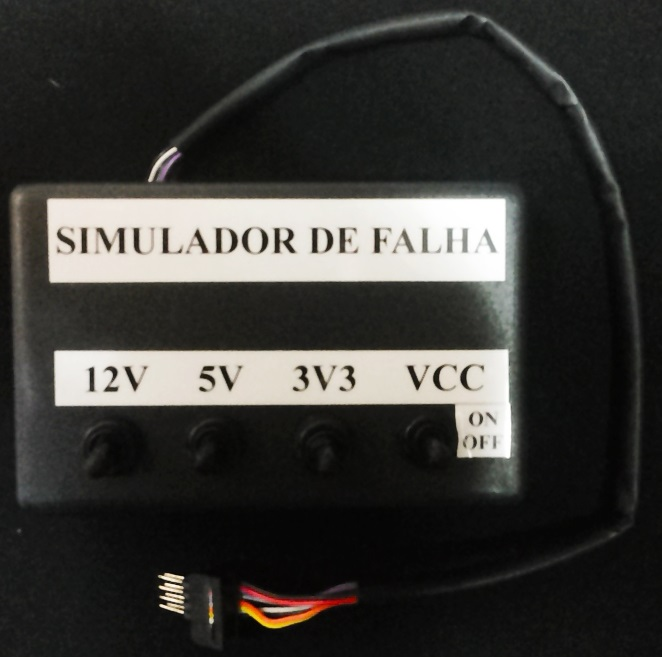
\includegraphics[width=0.4\linewidth]{./figs/Simulador}
			
		\begin{small}
			FONTE: Foto tirada pelos autores.
		\end{small}		
	\end{figure}
	\pagebreak

	Para que os conversores utilizados estejam em estado de operação é preciso ter uma tensão de 5V nos pinos de \textit{enable} dos circuitos integrados. Dessa forma as chaves \textit{ON/OFF} do simulador foram conectadas diretamente nesses pinos de \textit{enable}, conforme Figura \ref{Fig_Simulador_Enable}.
		
	\begin{figure}[th]
		\caption{CONEXÕES DO SIMULADOR DE FALHAS}
		\label{Fig_Simulador_Enable}
		\centering
		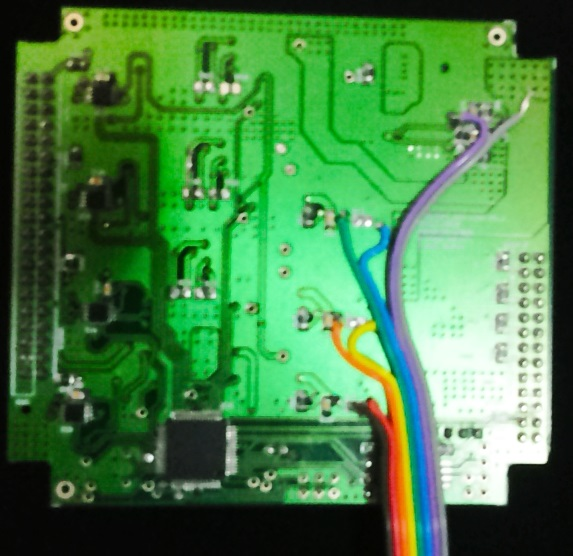
\includegraphics[width=0.5\linewidth]{./figs/simulador_conexao}
			
		\begin{small}
			FONTE: Foto tirada pelos autores.
		\end{small}		
	\end{figure}
	
	Como o circuito foi projetado para que os conversores principais (placa de controle) operem sempre com tensões pouco acima das tensões do conversor \textit{backup} (placa do carregador), as chaves ideais (TLC4412) estão sempre chaveadas para que a placa de controle forneça as tensões no barramento de saída. Para poder simular as falhas basta deixar o pino de \textit{enable} em aberto, dessa maneira é possível garantir a ausência da alimentação no circuito integrado. Essa operação fará com que a chave ideal identifique que a tensão do conversor \textit{backup} é maior do que a tensão do conversor principal, assim ela realiza o chaveamento para que o \textit{backup} forneça a tensão no barramento de saída.
	
	São dois os estados possíveis do simulador de falhas:
	
	\begin{itemize}
		\item[\textbf{\textit{ON}}] indica que a falha está ativa;
		\item[\textbf{\textit{OFF}}] indica que a falha está desativa. 
	\end{itemize}
	
	Na Tabela \ref{Tab_Simulador} é possível visualizar os estados de falha e a fonte responsável pela alimentação do barramento de saída.
	
	\begin{table}[th]
	\caption{SIMULAÇÃO DE FALHAS}
	\label{Tab_Simulador}
	\centering
		\begin{tabular}{p{1.5cm}|p{1.5cm}|p{5.5cm}}
			\textbf{Tensão} & \textbf{Falha} & \textbf{Barramento}\\
			\hline
			12V & \textit{OFF} & Conversor principal \\
			12V & \textit{ON} & Conversor \textit{backup} \\
			5V & \textit{OFF} & Conversor principal \\
			5V & \textit{ON} & Conversor \textit{backup} \\
			3,3V & \textit{OFF} & Conversor principal \\
			3,3V & \textit{ON} & Conversor \textit{backup} \\
			VCC & \textit{OFF} & Conversor principal dedicado \\
			VCC & \textit{ON} & Tensão do barramento \\
		\end{tabular}	
	
	\begin{small}
	\vspace{3pt}
		FONTE: Elaborada pelos autores.
	\end{small}
	\end{table}
	\pagebreak
	
	Com o objetivo de facilitar o monitoramento das simulações de falha foi criado no ambiente \textit{Simulink} uma interface de testes.
	
\subsection[Simulink]{\textit{Simulink}}

	O \textit{Simulink} é um ambiente de diagrama de blocos para a simulação de múltiplos domínios e de projetos de modelo baseado. É uma ferramenta integrada ao \textit{MatLab}.\textsuperscript{\cite{Simulink}}
	
	Com o objetivo de exibir os resultados dos testes realizados com o simulador de falhas, foi criado um \textit{software} supervisório no \textit{Simulink}. Os blocos utilizados foram dispostos de maneira a reproduzir o diagrama de blocos proposto, conforme Figura \ref{Fig_int}.
	
	\begin{figure}[th]
		\caption{INTERFACE CRIADA NO \textit{SIMULINK}}
		\label{Fig_int}
		\centering
		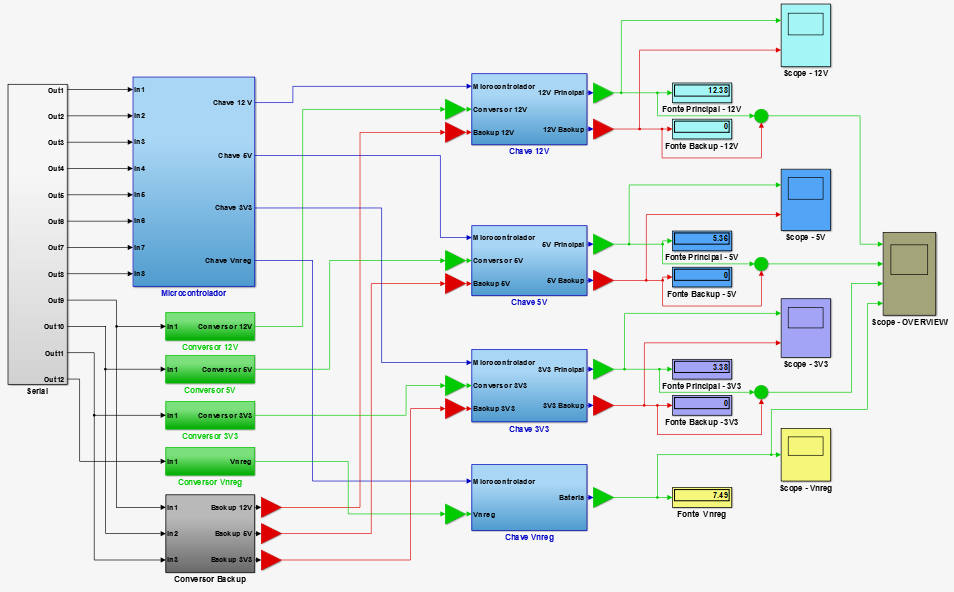
\includegraphics[width=1.0\linewidth]{./figs/int}
			
		\begin{small}
			FONTE: Elaborado pelos autores.
		\end{small}		
	\end{figure}
	
	Para que interface criada funcione corretamente é necessário que os seguintes complementos estejam instaladas:
	
	\begin{itemize}
		\item \textit{xPC Target};
		\item \textit{Instrument Control Toolbox};
		\item Compilador C.
	\end{itemize}

	O subsistema Serial contém todos os blocos responsáveis pela configuração de comunicação entre equipamento e supervisório, além de fazer a separação dos \textit{bytes} enviados para a correta distribuição na interface.
	
	O bloco do Microcontrolador, tem a função de distribuir o sinal responsável pelo controle das chaves ideais, que possuem a inteligência de controle automática além de poder ser controlada via microcontrolador.
	
	Os Conversores 12V, 5V, 3,3V e Vnreg são os responsáveis pelo envio das tensões lidas nos conversores da placa de controle, já o Conversor \textit{Backup} envia as tensões lidas no conversor da placa do carregador.
	
	Nos subsistemas das Chaves 12V, 5V, 3,3V e Vnreg existe uma lógica que faz a interpretação dos \textit{bytes} enviados pelos demais blocos, enviando o sinal recebido para os \textit{displays} das Fontes Principais e \textit{Backup}.
	
	O osciloscópio \textit{Scope - OVERVIEW} faz o monitoramento de todas as tensões do sistema indicando de forma gráfica todos os níveis de tensão em funcionamento, conforme Figura \ref{Fig_over}.
	
	\begin{figure}[th]
		\caption{MONITORAMENTO DO BARRAMENTO DE SAÍDA}
		\label{Fig_over}
		\centering
		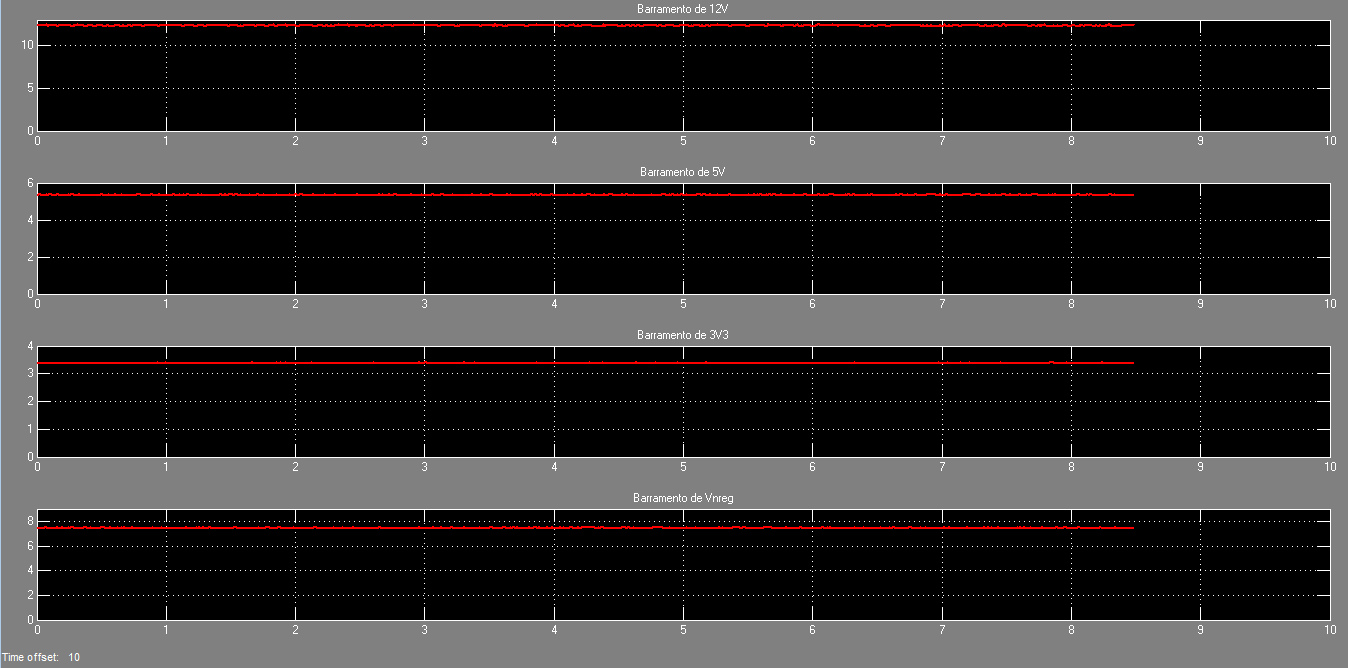
\includegraphics[width=1.0\linewidth]{./figs/over}
			
		\begin{small}
			FONTE: Foto tirada pelos autores.
		\end{small}		
	\end{figure}
	\pagebreak
	
	Além do \textit{Scope - OVERVIEW}, cada circuito de tensão possui um osciloscópio dedicado, neles é possível fazer o acompanhamento de uma tensão específica, dessa forma pode-se visualizar o valor da tensão no momento e qual a fonte que está fornecendo esse valor, além de identificar o momento do chaveamento entre as fontes, conforme Figura \ref{Fig_3v3}.
	
	\begin{figure}[th]
		\caption{MONITORAMENTO DAS FONTES DE 3,3V}
		\label{Fig_3v3}
		\centering
		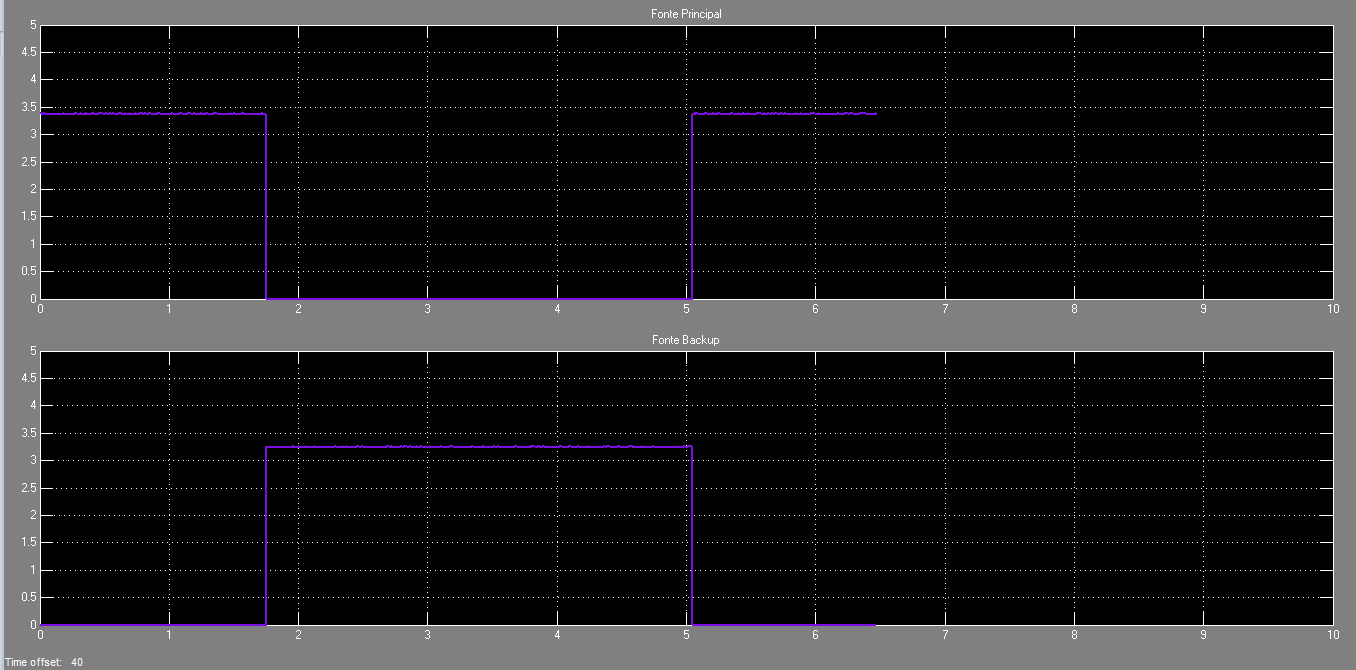
\includegraphics[width=1.0\linewidth]{./figs/3v3}
			
		\begin{small}
			FONTE: Foto tirada pelos autores.
		\end{small}		
	\end{figure}
	
	Na Figura \ref{Fig_ch} é exibido o monitoramento das fontes de 3,3V e o monitoramento do barramento de saída do Sistema de Gerenciamento de Energia para \textit{CubeSats}.
	
	\begin{figure}[th]
		\caption{VERIFICAÇÃO DA TENSÃO NO BARRAMENTO DURANTE CHAVEAMENTO DA FONTE}
		\label{Fig_ch}
		\centering
		\includegraphics[width=1.0\linewidth]{./figs/ch}
			
		\begin{small}
			FONTE: Foto tirada pelos autores.
		\end{small}		
	\end{figure}
	\pagebreak
	
	No supervisório foi criado também um algoritmo de animação que deixa as cores dos blocos dos conversores verde e vermelho, quando conversores ativos e desativos, respectivamente. Alguns computadores podem se perder enquanto executam o supervisório devido ao processamento das mensagens recebidas e a execução do \textit{script} utilizado nessa animação, nesses casos existe um supervisório adaptado que não contém o algoritmo de animação. 

	Nesse capítulo foi abordado o princípio de funcionamento do Sistema de Gerenciamento de Energia para \textit{CubeSats}, os parâmetros utilizado para realizar a selação dos componentes e os métodos adotados na construçao da solução proposta. No capítulo a seguir, será abordado os resultados obtidos e as discussões que giram em torno do projeto.
	
	
% ----------------------------------------------------------
% RESULTADOS E DISCUSSÕES
% ----------------------------------------------------------
\chapter[Resultados e discussões]{Resultados e discussões}

	Nesse capítulo será apresentado os resultados obtidos nos testes de validação e uma breve explanação sobre o resultado geral do Sistema de Gerenciamento de Energia.
	
\section[Ensaios realizados]{Ensaios realizados}

	Alguns testes foram realizados para aferir o funcionamento dos circuitos, dentre os ensaios possíveis foram realizados:
	
	\begin{itemize}
	\item Individual da fotocélula;
		\item Conjunto de fotocélulas;
		\item Conversor principal de 5V;
		\item Conversor principal de 12V;
		\item Chave ideal para 5V.		
	\end{itemize}
	
\subsection[Ensaio individual de fotocélula]{Ensaio individual de fotocélula}

	O ensaio individual de fotocélula foi realizado variando a resistência de carga entre 1$\Omega$ e 200$\Omega$, o resultado do ensaio e a comparação com os dados teóricos podem ser visualizados graficamente na Figura \ref{Fig_ens_cell}.
	
	\begin{figure}[th]
		\caption{COMPARATIVO DOS RESULTADOS PRÁTICOS E DE \textit{DATASHEET}}
		\centering
		\label{Fig_ens_cell}
		\includegraphics[width=0.7\linewidth]{./figs/ens_cell}
		
		\begin{small}
			FONTE: Elaborado pelos autores.
		\end{small}	
	\end{figure}

	Devido as condições de testes, os resultados de \textit{datasheet} e prático possuem valores divergentes. Porém ao observar a curva nota-se um comportamento semelhante entre os ensaios, ressaltando que os valores fornecidos na especificação foram obtidos de ensaios com ambiente controlado, diferente dos ensaios realizados para aferição do painel solar.
	
	
\subsection[Ensaio do conjunto de fotocélulas]{Ensaio do conjunto de fotocélulas}

	O ensaio do conjunto de fotocélulas foi realizado variando a resistência de carga entre 500$\Omega$ e 5k$\Omega$, o resultado do ensaio pode ser visualizado na Figura \ref{Fig_ens_cell4}.\footnote{No Apêndice \ref{An_cell4}, é possível verificar a tabela com os dados do ensaio.} 
	
	\begin{figure}[th]
		\caption{ENSAIO DO CONJUNTO DE FOTOCÉLULAS}
		\centering
		\label{Fig_ens_cell4}
		\includegraphics[width=1.0\linewidth]{./figs/ens_cell4}
		
		\begin{small}
			FONTE: Elaborado pelos autores.
		\end{small}	
	\end{figure}
	
	É possível notar no ensaio dos conjuntos de fotocélulas que existe uma clara variação entre as amostras, não sendo obtido um resultado uniforme, esse resultado se deve, provavelmente, ao processo de soldagem no forno e a manipulação inadequada do material com as mãos.
	
\subsection[Ensaio do conversor principal de 5V]{Ensaio do conversor principal de 5V}

	Conforme o esquema de testes apresentado na Figura \ref{Fig_esq_cont}, foram obtidos os resultados apresentados na Figura \ref{Fig_rend5}.
	
	\begin{figure}[th]
		\caption{RENDIMENTO APRESENTADO PELO CONVERSOR 5V}
		\label{Fig_rend5}
		\centering
		\includegraphics[width=0.9\linewidth]{./figs/rend5}
			
		\begin{small}
			FONTE: Elaborado pelos autores.
		\end{small}		
	\end{figure}
	
	
	Para os ensaios realizados foram obtidos os rendimentos exibidos na Tabela \ref{Tab_rend5}.
	
	\begin{table}[th]
	\caption{RENDIMENTO DO CONVERSOR DE 5V}
	\label{Tab_rend5}
	\centering
		\begin{tabular}{p{2cm}|p{4cm}}
			\textbf{Condição} & \textbf{Rendimento médio}\\
			\hline
			7,4V & 95,46\%\\
			8,0V & 95,22\%\\
			8,4V & 93,53\%\\
		\end{tabular}	
	
	\begin{small}
	\vspace{3pt}
		FONTE: Elaborada pelos autores.
	\end{small}
	\end{table}
	
	O rendimento obtido no conversor principal de 5V (TPS563200) foi de encontro com a informação fornecida no \textit{datasheet} do componente, por volta de 95\%.\footnote{No Apêndice \ref{An_rend5}, é possível verificar a tabela com os dados do ensaio.} 

\subsection[Ensaio do conversor principal de 12V]{Ensaio do conversor principal de 12V}

	Para realizar o ensaio do conversor principal de 12V, foi realizado o mesmo procedimento para o teste do conversor de 5V, apresentando os resultados exibidos na Figura \ref{Fig_rend12}
	
	\begin{figure}[th]
		\caption{RENDIMENTO APRESENTADO PELO CONVERSOR 12V}
		\label{Fig_rend12}
		\centering
		\includegraphics[width=0.9\linewidth]{./figs/rend12}
			
		\begin{small}
			FONTE: Elaborado pelos autores.
		\end{small}		
	\end{figure}	
	
	Para os ensaios realizados foram obtidos os rendimentos exibidos na Tabela \ref{Tab_rend12}.
	
	\begin{table}[th]
	\caption{RENDIMENTO DO CONVERSOR DE 12V}
	\label{Tab_rend12}
	\centering
		\begin{tabular}{p{2cm}|p{4cm}}
			\textbf{Condição} & \textbf{Rendimento médio}\\
			\hline
			7,4V & 90,29\%\\
			8,0V & 90,94\%\\
			8,4V & 90,92\%\\
		\end{tabular}	
	
	\begin{small}
	\vspace{3pt}
		FONTE: Elaborada pelos autores.
	\end{small}
	\end{table}
	
	O rendimento obtido no conversor principal de 12V (LT1941) foi de encontro com a informação fornecida no \textit{datasheet} do componente, por volta de 90\%.\footnote{No Apêndice \ref{An_rend12}, é possível verificar a tabela com os dados do ensaio.} 
	
	\subsection[Chave ideal do 5V]{Chave ideal do 5V}

	Para a validação da chave ideal do 5V, foi realizado um ensaio que consistia em validar o funcionamento da chave e obter o rendimento das chaves, o que pode ser visualizado na Figura \ref{Fig_rendch5}.
	
	\begin{figure}[th]
		\caption{RENDIMENTO APRESENTADO PELA CHAVE IDEAL DO 5V}
		\label{Fig_rendch5}
		\centering
		\includegraphics[width=0.8\linewidth]{./figs/rendch5}
			
		\begin{small}
			FONTE: Elaborado pelos autores.
		\end{small}		
	\end{figure}

	Para os ensaios realizados foram obtidos os rendimentos exibidos na Tabela \ref{Tab_rendch5}.
	
	\begin{table}[th]
	\caption{RENDIMENTO DA CHAVE IDEAL DO 5V}
	\label{Tab_rendch5}
	\centering
		\begin{tabular}{p{2cm}|p{4cm}}
			\textbf{Fonte} & \textbf{Rendimento médio}\\
			\hline
			Principal & 96,25\%\\
			\textit{Backup} & 96,23\%\\
		\end{tabular}	
	
	\begin{small}
	\vspace{3pt}
		FONTE: Elaborada pelos autores.
	\end{small}
	\end{table}

	Os resultados obtidos comprovam que as chaves ideias (LTC4412) utilizadas são de baixas perdas, o que reforça a robutez do sistema garantindo sempre o melhor desempenho na tensão fornecida no barramento.\footnote{No Apêndice \ref{An_rendch5}, é possível verificar a tabela com os dados do ensaio.} 
	
\section[Protótipo]{Protótipo}

	Como o \textit{CubeSat} Mauá é um projeto multidisciplinar, cada um dos subsistemas foram desenvolvidos separadamente para serem integrados após as devidas validações. Dessa forma foi desenvolvido um protótipo de uma unidade dedicada ao Sistema de Gerenciamento de Energia para \textit{CubeSats}.	
	
	As placas de controle e do carregador ficaram fixadas nas arestas do cubo deixando a parte interna disponível, aumentando a área livre para a carga útil. Esse formato de construção foi um diferencial implementado no projeto, uma vez que na maioria dos \textit{CubeSats} as placas são colocadas de forma horizontal no interior do cubo, dispostas como um \textit{rack}.
	
	Na Figura \ref{Fig_cube} é possível visualizar o protótipo da unidade do Sistema de Gerenciamento de Energia do \textit{CubeSat} Mauá.
	
	\begin{figure}[th]
		\caption{\textit{CUBESAT} MAUÁ}
		\label{Fig_cube}
		\centering
		\includegraphics[width=0.5\linewidth]{./figs/cube}
			
		\begin{small}
			FONTE: Foto tirada pelos autores.
		\end{small}
		
		\begin{footnotesize}
			NOTA: Painéis solares meramente ilustrativos.
		\end{footnotesize}
	\end{figure}
	
	

% ----------------------------------------------------------
% CONCLUSÕES
% ----------------------------------------------------------
\chapter[Conclusões e sugestões para trabalhos futuros]{Conclusões e sugestões para trabalhos futuros} \label{ultimo_capitulo}

	A seguir será apresentada a conclusão do projeto desenvolvido e sugestões para trabalhos futuros.
	
\section[Conclusões gerais]{Conclusões gerais}

	Frente aos objetivos traçados inicialmente durante os estudos deste trabalho, o resultado foi alcançado parcialmente. O foco principal do sistema ficou sobre o estudo de potência, com os conversores CC/CC onde foi possível obter altas eficiências de conversão de energia com a utilização de componentes comerciais.
	
	 Dentre as dificuldades encontradas para o desenvolvimento do projeto, a falta de fornecedores sediados no Brasil, resultou na importação de todos os componentes utilizados, que devido a logística necessária para a entrega deles afetou no tempo que seria dedicado aos ensaios. A burocracia no processo de aprovação das compras também impactou nesse processo.
	 
	 A solução implementada para a aumentar a vida útil do Sistema de Gerenciamento de Energia, utilizando uma fonte \textit{backup} se montou bastante eficaz, o chaveamento entre as fontes de energia principal e \textit{backup} com o uso de chaves ideal se mostrou bastante funcional por apresentar baixa perda e não ocasionar pertubações a carga, que continua operando normalmente. 
	
	O sistema da forma que foi implementado se tornar uma plataforma didática para estudos de eletrônica de potência na área aeroespacial, respeitando as normas especificadas pela \textit{Cal Poly}. 

	As redundâncias funcionaram como projetado pelo grupo, fazendo com que caso o conversor principal diminua sua tensão, a ponto de ficar a baixo da tensão fornecida pelo conversor \textit{backup}, este toma seu lugar e começa, imediatamente, a fornecer a energia no barramento de saída, sem que a carga sinta a comutação entre as fontes. Isso ocorre individualmente para cada um dos conversores ou até para todos juntos, não prejudicando o fornecimento de energia aos demais subsistemas do \textit{CubeSat}.

	Os tópicos que se destacaram no desenvolvimento do projeto foram:
	
	\begin{itemize}
		\item Alta eficiência atingida com conversores de baixo custo;
		\item Fontes de redundância de alta eficiência;
		\item Chaveamento instantâneo entre fontes;
		\item Utilização de componentes de fácil acesso;
		\item Otimização da área útil do \textit{CubeSat};
		\item Desenvolvimento de \textit{software} supervisório;
		\item Desenvolvimento de um simulador de falhas.
	\end{itemize}

\section[Sugestões para trabalhos futuros]{Sugestões para trabalhos futuros}
	
	Como o objetivo do \textit{CubeSat} Mauá é ser lançado e também tornar-se um projeto de estudo constante do NSEE, alguns pontos do projeto podem ser melhorados, sendo eles:
	
	\begin{itemize}
		\item Realizar os ensaios de determinação do rendimento no conversor principal de 3,3V e no conversor \textit{backup};
		\item Montagem e ensaio do sistema de carregamento de bateria;
		\item Ensaio do painel solar;
		\item Implementar a comunicação CAN;
		\item Desenvolver um processo estruturado para a realização dos ensaios de radiação e termovácuo;\footnote{No Apêndice \ref{ensaios}, é possível ver mais informações sobre os ensaios propostos.}
		\item Integração com demais subsistemas.
	\end{itemize}
	
% ----------------------------------------------------------
% REFERÊNCIAS BIBLIOGRÁFICAS
% ----------------------------------------------------------
\bibliography{TCC_Sist_Gerenciamento_Potencia}

% ----------------------------------------------------------
% Apêndices
% ----------------------------------------------------------

% ---
% Inicia os Apêndices
% ---
\begin{apendicesenv}

% Imprime uma página indicando o início dos Apêndices
\partapendices

% ---
\chapter[Orçamento dos componentes da Farnell]{Orçamento dos componentes da \textit{Farnell}} \label{Orçamento}


	Orçamento enviado pelo Sr. Helder Sant'ana Viana da \textit{Farnell Newark element14}.

	\begin{figure}[th]
		\centering
		\includegraphics[width=0.85\linewidth]{./anexos/Pedido189845}	
	\end{figure}
	
	\begin{figure}[th]
		\centering
		\includegraphics[width=0.9\linewidth]{./anexos/Pedido1898452}	
	\end{figure}
	
	\begin{figure}[th]
		\centering
		\includegraphics[width=0.9\linewidth]{./anexos/Pedido1898453}	
	\end{figure}
	
\chapter[Forno de refusão ProtoFlow E]{Forno de refusão \textit{ProtoFlow E}} \label{ProtoFlow}
	
	\begin{figure}[th]
		\caption{FORNO DE REFUSÃO \textit{PROTOFLOW E}}
		\centering
		\includegraphics[width=0.75\linewidth]{./anexos/proto1}
		
		\begin{small}
			FONTE: Foto tirada pelos autores.
		\end{small}	
	\end{figure}
	
	\begin{figure}[th]
		\caption{PROCESSO DE ESTANHAMENTO DOS \textit{PADS} DAS FOTOCÉLULAS}
		\centering
		\includegraphics[width=0.75\linewidth]{./anexos/proto2}
		
		\begin{small}
			FONTE: Foto tirada pelos autores.
		\end{small}	
	\end{figure}
	
	\begin{figure}[th]
		\caption{CURVA DE TEMPERATURA DO PROCESSO DE SOLDAGEM}
		\centering
		\includegraphics[width=0.75\linewidth]{./anexos/configproto}
		
		\begin{small}
			FONTE: Elaborado pelos autores.
		\end{small}		
	\end{figure}
	
	\begin{figure}[th]
		\caption{PAINEL SOLAR EM PROCESSO DE SOLDAGEM}
		\centering
		\includegraphics[width=0.75\linewidth]{./anexos/proto3}
		
		\begin{small}
			FONTE: Foto tirada pelos autores.
		\end{small}	
	\end{figure}
	
	\begin{figure}[th]
		\caption{PROCESSO DE RESFRIAMENTO DO PAINEL SOLAR}
		\centering
		\includegraphics[width=0.75\linewidth]{./anexos/proto4}
		
		\begin{small}
			FONTE: Foto tirada pelos autores.
		\end{small}	
	\end{figure}
	

\chapter[Placa do carregador]{Placa do carregador}\label{P_Carreg}

	\begin{figure}[th]
		\caption{\textit{LAYOUT} DA PLACA DO CARREGADOR}
		\centering
		\includegraphics[width=0.75\linewidth]{./anexos/placa_carreg}
		
		\begin{small}
			FONTE: Elaborado pelos autores.
		\end{small}	
	\end{figure}	
	
	
\chapter[Placa de controle]{Placa de controle}\label{P_Cont}

	\begin{figure}[th]
		\caption{\textit{LAYOUT} DA PLACA DE CONTROLE}
		\centering
		\includegraphics[width=0.75\linewidth]{./anexos/placa_cont}
		
		\begin{small}
			FONTE: Elaborado pelos autores.
		\end{small}	
	\end{figure}
	
\chapter[Pontos de teste da placa de controle]{Pontos de teste da placa de controle}\label{T_Cont}

	\begin{figure}[th]
		\caption{PONTOS DE TESTE DA PLACA DE CONTROLE}
		\centering
		\includegraphics[width=0.75\linewidth]{./anexos/t_cont}
		
		\begin{small}
			FONTE: Elaborado pelos autores.
		\end{small}	
	\end{figure}
	
\chapter[Protocolo de comunicação]{Protocolo de comunicação}\label{Prot_Serial}

	O protocolo de comunicação serial \textit{topx} possui a seguinte estrutura:

	\begin{enumerate}
		\item Identificação da tensão de 12V;
		\item Identificação de fonte principal ou \textit{backup};
		\item Primeiro dígito da tensão de 12V;
		\item Segundo dígito da tensão de 12V;
		\item Terceiro dígito da tensão de 12V;
		\item Quarto dígito da tensão de 12V;
		\item Identificação da tensão de 5V;
		\item Identificação de fonte principal ou \textit{backup};
		\item Primeiro dígito da tensão de 5V;
		\item Segundo dígito da tensão de 5V;
		\item Terceiro dígito da tensão de 5V;
		\item Quarto dígito da tensão de 5V;
		\item Identificação da tensão de 3,3V;
		\item Identificação de fonte principal ou \textit{backup};
		\item Primeiro dígito da tensão de 3,3V;
		\item Segundo dígito da tensão de 3,3V;
		\item Terceiro dígito da tensão de 3,3V;
		\item Quarto dígito da tensão de 3,3V;
		\item Identificação da tensão de V$ _{nreg} $;
		\item Identificação de fonte principal ou \textit{backup};
		\item Primeiro dígito da tensão de V$ _{nreg} $;
		\item Segundo dígito da tensão de V$ _{nreg} $;
		\item Terceiro dígito da tensão de V$ _{nreg} $;
		\item Quarto dígito da tensão de V$ _{nreg} $;
		\item Terminador.
	\end{enumerate}
	
\chapter[Resultados do ensaio realizado no conjunto de fotocélulas]{Resultados do ensaio realizado no conjunto de fotocélulas}\label{An_cell4}

	\begin{figure}[th]
		\caption{RESULTADOS OBTIDOS NO PAINEL SOLAR}
		\centering
		\includegraphics[width=0.35\linewidth]{./anexos/cell4}
		
		\begin{small}
			FONTE: Elaborado pelos autores.
		\end{small}	
	\end{figure}
	
\chapter[Resultados do ensaio realizado no conversor de 5V]{Resultados do ensaio realizado no conversor de 5V}\label{An_rend5}

	\begin{figure}[th]
		\caption{RESULTADOS OBTIDOS NO CONVERSOR DE 5V}
		\centering
		\includegraphics[width=0.75\linewidth]{./anexos/rend5_1}
		
		\begin{small}
			FONTE: Elaborado pelos autores.
		\end{small}	
		
		\begin{footnotesize}
		NOTA: Ensaio realizado com bateria descarregada (7,4V)
		\end{footnotesize}
	\end{figure}
	
	\begin{figure}[th]
		\caption{RESULTADOS OBTIDOS NO CONVERSOR DE 5V}
		\centering
		\includegraphics[width=0.75\linewidth]{./anexos/rend5_2}
		
		\begin{small}
			FONTE: Elaborado pelos autores.
		\end{small}	
		
		\begin{footnotesize}
		NOTA: Ensaio realizado com bateria carregada (8,0V)
		\end{footnotesize}
	\end{figure}
	
	\begin{figure}[th]
		\caption{RESULTADOS OBTIDOS NO CONVERSOR DE 5V}
		\centering
		\includegraphics[width=0.75\linewidth]{./anexos/rend5_3}
		
		\begin{small}
			FONTE: Elaborado pelos autores.
		\end{small}	
		
		\begin{footnotesize}
		NOTA: Ensaio realizado com bateria completamente carregada (8,4V)
		\end{footnotesize}
	\end{figure}
	
\chapter[Resultados do ensaio realizado no conversor de 12V]{Resultados do ensaio realizado no conversor de 12V}\label{An_rend12}

	\begin{figure}[th]
		\caption{RESULTADOS OBTIDOS NO CONVERSOR DE 12V}
		\centering
		\includegraphics[width=0.75\linewidth]{./anexos/rend12_1}
		
		\begin{small}
			FONTE: Elaborado pelos autores.
		\end{small}	
		
		\begin{footnotesize}
		NOTA: Ensaio realizado com bateria descarregada (7,4V).
		\end{footnotesize}
	\end{figure}
	
	\begin{figure}[th]
		\caption{RESULTADOS OBTIDOS NO CONVERSOR DE 12V}
		\centering
		\includegraphics[width=0.75\linewidth]{./anexos/rend12_2}
		
		\begin{small}
			FONTE: Elaborado pelos autores.
		\end{small}	
		
		\begin{footnotesize}
		NOTA: Ensaio realizado com bateria carregada (8,0V).
		\end{footnotesize}
	\end{figure}
	
	\begin{figure}[th]
		\caption{RESULTADOS OBTIDOS NO CONVERSOR DE 12V}
		\centering
		\includegraphics[width=0.75\linewidth]{./anexos/rend12_3}
		
		\begin{small}
			FONTE: Elaborado pelos autores.
		\end{small}	
		
		\begin{footnotesize}
		NOTA: Ensaio realizado com bateria completamente carregada (8,4V).
		\end{footnotesize}
	\end{figure}	
	
\chapter[Resultados do ensaio realizado na chave ideal do 5V]{Resultados do ensaio realizado na chave ideal do 5V}\label{An_rendch5}

	\begin{figure}[th]
		\caption{RESULTADOS OBTIDOS NA CHAVE IDEAL DO 5V}
		\centering
		\includegraphics[width=0.75\linewidth]{./anexos/chavep}
		
		\begin{small}
			FONTE: Elaborado pelos autores.
		\end{small}	
		
		\begin{footnotesize}
		NOTA: Ensaio realizado com chave fornecendo tensão do conversor principal.
		\end{footnotesize}
	\end{figure}
	
	\begin{figure}[th]
		\caption{RESULTADOS OBTIDOS NA CHAVE IDEAL DO 5V}
		\centering
		\includegraphics[width=0.75\linewidth]{./anexos/chaveb}
		
		\begin{small}
			FONTE: Elaborado pelos autores.
		\end{small}	
		
		\begin{footnotesize}
		NOTA: Ensaio realizado com chave fornecendo tensão do conversor \textit{backup}.
		\end{footnotesize}
	\end{figure}
	
\chapter[Ensaios futuros]{Ensaios futuros}\label{ensaios}
	
\section[Ensaio de radiação]{Ensaio de radiação}	

	O ensaio de radiação consiste na emissão de radiação nos semicondutores a fim de se obter a assinatura da tensão e corrente após a exposição a radiação. Para esse ensaio é necessário que os semicondutores estejam decapados, ou seja, é necessário que a dopagem de sílicio do semicondutor fique exposta para que a emissão da radiação seja direta no componente, fato que não ocorrerá no espaço, uma vez que a película do componente estará presente o que, por sua vez, acaba dando uma pequena filtrada na radiação. Esse teste pode ser realizado em conjunto com o Centro Universitário da Faculdade de Engenharia Industrial (FEI), com a Dr. Marcilei Guazzelli da FEI.	
	
\section[Ensaio térmico]{Ensaio térmico}

	O ensaio térmico pode ser realizado em parceria com o laboratório da USP, coordenado pelo Dr. Fábio Rodrigues. Esse ensaio consiste em uma câmara refrigerada que atinge uma temperatura próxima aos -80 ºC. 

\section[Ensaio de vácuo]{Ensaio de vácuo}	

	O ensaio térmico pode ser realizado em parceria com o laboratório da USP, coordenado pelo Dr. Fábio Rodrigues. Esse ensaio consiste em uma câmara de vácuo que atinge uma pressão de aproximadamente 10\textsuperscript{-9} mbar. 
	
\section[Ensaio de termovácuo]{Ensaio de termovácuo}

	Por fim, após todas as validações anteriores os subconjuntos podem ser enviados para Vinhedo no Observatório Abrahão de Moraes onde o Dr. Douglas Galante, poderá realizar o ensaio de termovácuo.
	
	\begin{figure}[th]
		\caption{CÂMERA DE TERMOCÁCUO}
		\label{Fig_SubConj}
		\centering
		\includegraphics[width=0.5\linewidth]{./figs/termovacuo}
			
		\begin{small}
			FONTE: Foto tirada pelos autores.
		\end{small}		
	\end{figure}
	\pagebreak
	
	Nesse ensaio é possível atingir baixas pressões (10\textsuperscript{-9} mbar) e também baixas temperaturas, sendo possível visualizar no \textit{LabView} a curva da pressão, onde é fácil constatar se algum problema ocorreu caso na curva tenha alguma subida repentina de pressão.
	
	\begin{figure}[th]
		\caption{CURVA DE PRESSÃO NO \textit{LABVIEW}}
		\label{Fig_SubConj}
		\centering
		\includegraphics[width=0.8\linewidth]{./figs/labview}
			
		\begin{small}
			FONTE: Foto tirada pelos autores.
		\end{small}		
	\end{figure}
	
	
\end{apendicesenv}



% ----------------------------------------------------------
% 
% ----------------------------------------------------------
%\chapter[]{}









%---------------------------------------------------------------------
% INDICE REMISSIVO
%---------------------------------------------------------------------
\phantompart
\printindex
%---------------------------------------------------------------------


\end{document}
